\documentclass[12pt,a4paper]{article}

\usepackage{graphicx}
\usepackage{subcaption}
\usepackage{booktabs}
\usepackage{multirow}
\usepackage{array}
\usepackage{float}
\usepackage{amsmath}
\usepackage{amsfonts}
\usepackage[backend=biber, style=numeric, sorting=none]{biblatex}
\usepackage[linesnumbered,ruled,vlined]{algorithm2e}
\usepackage{hyperref}
\addbibresource{bibliography.bib} % Specify the .bib file


\setlength{\topmargin}{0.0in}
\setlength{\oddsidemargin}{0.33in}
\setlength{\textheight}{9.0in}
\setlength{\textwidth}{6.0in}
\renewcommand{\baselinestretch}{1.25}


\title{Brownian Microswimmers: Investigating models that capture boundary accumulation of microorganisms}

\author{Inti-Raymi Carhuancho Mantripp}
\date{Candidate Number: 1090497}

\begin{document}

\maketitle

\thispagestyle{empty}

\newpage
\setcounter{page}{1}


\section{Introduction}\label{sec: intro}
Many types of self-propelled microorganisms moving through water tend to accummulate near the boundaries
of their environments. This has been observed both experimentally, \cite{rothschild1963non}, 
\cite{berke2008hydrodynamic} and in nature. Figure \ref{fig:both_images} shows two characteristic
illustrations of this behaviour by plotting the density cells and bacteria observed cross-sectionally 
within their domains.

\begin{figure}[htbp]\label{fig: intro_distributions}
    \centering
    \begin{subfigure}[b]{0.45\textwidth}
      \centering
      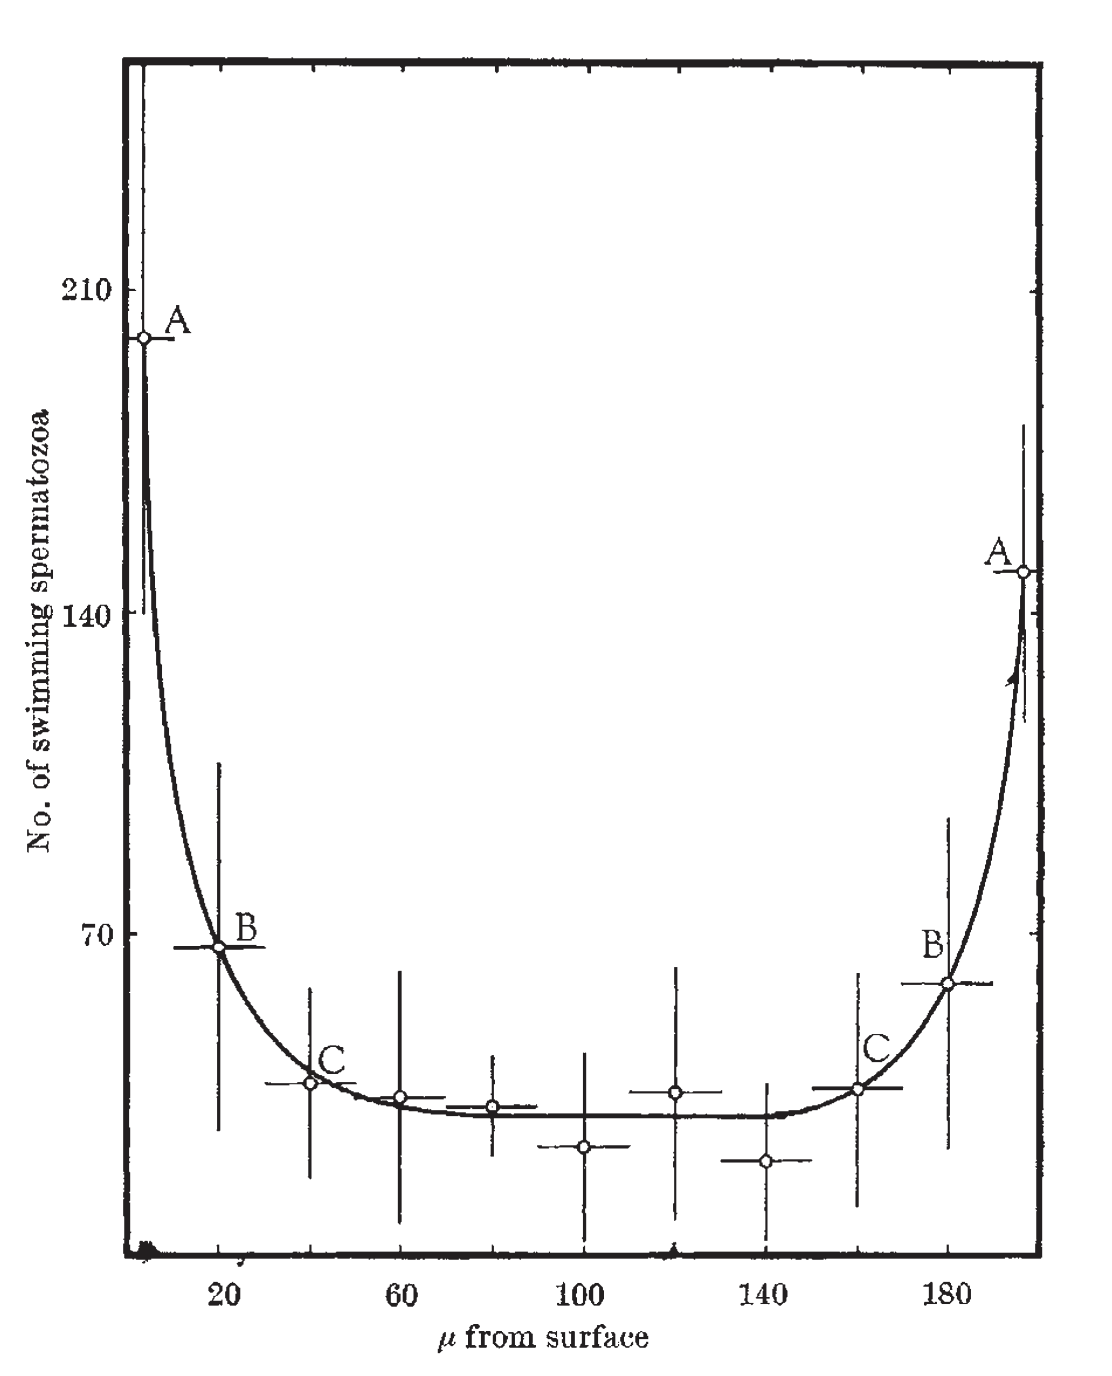
\includegraphics[width=\textwidth]{graphics/bull_spermatazoa_ distribution.png}
      \caption{Distribution of bull spermatazoa in suspended medium \cite{rothschild1963non}.}
      \label{fig:image1}
    \end{subfigure}
    \hfill
    \begin{subfigure}[b]{0.45\textwidth}
      \centering
      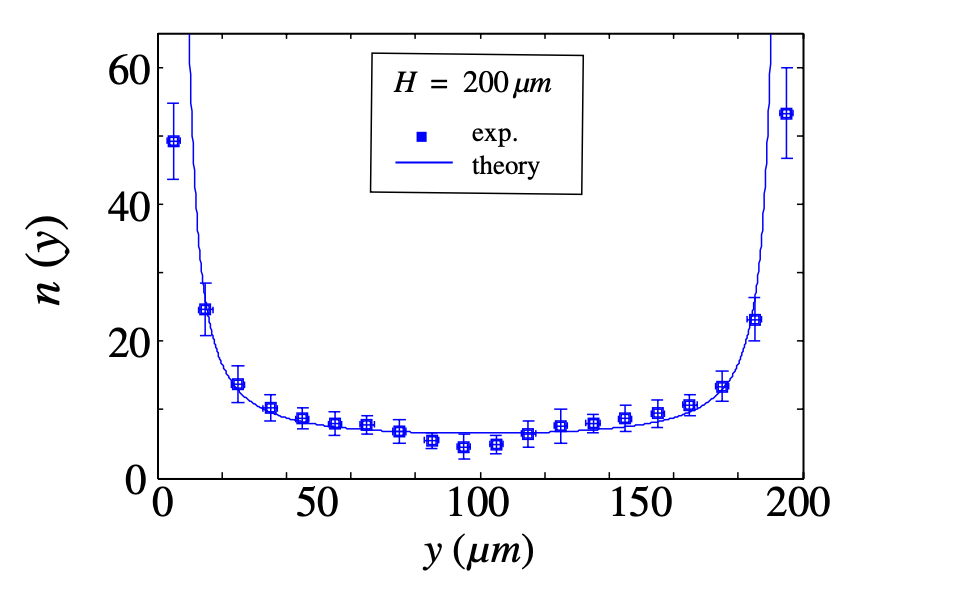
\includegraphics[width=\textwidth]{graphics/e_coli_distribution.png}
      \caption{Distribution of E. coli bacteria between two glass plate \cite{berke2008hydrodynamic}.}
      \label{fig:image2}
    \end{subfigure}
    \caption{Experimental results illustrating boundary accummulation of swimming microorganisms.}
    \label{fig:both_images}
  \end{figure}

Many models have been proposed to describe the behaviour of microswimmers(\cite{chen2021shape},
\cite{berke2008hydrodynamic}, \cite{ai2013rectification}), and this observed boundary accummulation is
an important feature for such models to capture. The purpose of such models is not only to describe this behaviour
but also to provide some explanation behind it.


The goal of this report is to present three models that describe the behaviour of swimming microorganisms,
with a particular focus on capturing the observed boundary accummulation. Before introducing these models, 
a brief overview of stochastic PDEs and the Fokker-Planck equation will be given.

The structure of this report is as follows:


\section{Main}\label{sec:2_models_and_preamble}
The dynamics of microorganisms are in part the result of microscopic interactions between organisms and their
surrounding environment SOURCE NEEDED. Rather than model this directly, this is typically captured by introducing
stochastic terms to their dynamics. This is done in all the models covered in this report, and for that reason we will give an 
overview of stochastic differential equations (SDEs) followed by their solution via the Monte Carlo methods and the
Fokker-Planck equation.

\subsection{Stochastic Differential Equations and the Fokker-Planck Equation}
For the purposes of this report, SDEs can be conceptually viewed as differential equations
with an additional random term that introduces stochastic fluctuations to their dyamics. 

To illustrate, consider the deterministic differential equation:

\begin{equation*}
    dx = \mu(x(t),t)dt.
\end{equation*}

Here, $x(t)$ is a deterministic variable with a drift term $\mu(x(t), t)$, mapping $\mathbb{R} \times[0, \infty) \to \mathbb{R}$. 
By adding stochasticity through Brownian motion

\begin{equation}\label{eq:sde}
    dX = \mu(X(t),t)dt + \sigma(X(t), t)dW
\end{equation}

where $X(t)$ is now a stochastic process. Here, $\mu(X(t), t)dt$ continues to be the deterministic drift term, while
$\sigma(X_t, t)$ is known as the \textit{diffusion term}, scaling the stochastic fluctuations introduced by the 
Wiener process $W_t$. The increments of $W_t$ are normally distributed as follows:

\begin{equation*}
    dW \sim \mathcal{N}(0, dt).
\end{equation*}

By selecting a sufficiently small time step $\Delta t$, we discretise equation \eqref{eq:sde} to 
numerically approximate the differential as:

\begin{equation}\label{eq:differential_approximation}
    \Delta X = \mu(X(t), t)\Delta t + \sigma(X(t), t) \Delta W
\end{equation}

Equation \eqref{eq:differential_approximation} can be used in an iterative approach to obtain a 
sample trajectory of the SDE in equation \eqref{eq:sde}:

\begin{equation}\label{eq:forward_euler}
    X(t + \Delta t) = X(t) + \Delta X.
\end{equation}

This method is called the Euler-Maruyama method, a stochastic
analogue of the forward Euler method \cite{erban2020stochastic}. 

As $X(t)$ is a stochastic process, 
at any fixed time $t$, $X(t)$ has a distribution described by its 
probability distribution function (PDF).
To obtain the PDF of the random variable $X(t)$ at a given time $t$, two main approaches exist. Firstly, using
the Euler-Maruyama method one can generate
$n$ independent trajectories of the SDE. Provided $n$ is sufficiently large, one can construct 
an empirical density from the realisations of $X(t)$ at time $t$. This approach is called the Monte Carlo method, 
and its accuracy depends on the number of samples $n$. By the central limit theorem, the error in 
estimating the PDF decreases like:

\begin{equation*} 
    \text{Error} \sim \mathcal{O}(n^{-1/2}). 
\end{equation*}


This means that to halve the error we must quadruple the number of samples. This can make Monte Carlo methods
computationally expensive for high precision estimates. 

An alternative approach to determining the PDF is through the Fokker-Planck equation.
The Fokker-Planck equatino is a partial differenial equation (PDE) describing the evolution of the PDF $p(x, t)$ 
associated with $X(t)$. For the SDE given in equation \eqref{eq:sde}, the corresponding Fokker-Planck equation is:

\begin{equation}
    \frac{\partial p(x,t)}{\partial t} = -\frac{\partial}{\partial x}\left[ \mu(x,t) p(x,t) \right] + \frac{1}{2}\frac{\partial^2}{\partial x^2}\left[ \sigma^2(x,t) p(x,t) \right],
\end{equation}

where $p(x,t)$ is the probability density function of the random variable $X_t$. 
Solving this PDE can directly yield the PDF without the sampling noise inherent in Monte Carlo simulations.

For systems involving multiple interacting stochastic processes, we consider a system of coupled SDEs:

\begin{equation}
    d\mathbf{X}_t = \boldsymbol{\mu}(\mathbf{X}_t, t),dt + \boldsymbol{\Sigma}(\mathbf{X}_t, t), d\mathbf{W}_t,
\end{equation}

where $\mathbf{X}_t \in \mathbb{R}^n$ is a vector-valued stochastic process, $\boldsymbol{\mu}(\mathbf{X}_t, t)$ 
is a vector of drift terms, $\boldsymbol{\Sigma}(\mathbf{X}_t, t)$ is a diffusion matrix, and 
$\mathbf{W}_t \in \mathbb{R}^m$ is a vector of independent Wiener processes. The associated Fokker-Planck
equation describing the evolution of the joint probability density $p(\mathbf{x}, t)$ for the system is given by:

\begin{equation}
    \frac{\partial p(\mathbf{x}, t)}{\partial t} = -\nabla_{\mathbf{x}} \cdot \left[ \boldsymbol{\mu}(\mathbf{x}, t) p(\mathbf{x}, t) \right] 
    + \frac{1}{2} \nabla_{\mathbf{x}} \cdot \left( \nabla_{\mathbf{x}} \cdot \left[ \boldsymbol{\Sigma}(\mathbf{x}, t) \boldsymbol{\Sigma}(\mathbf{x}, t)^T p(\mathbf{x}, t) \right] \right).
\end{equation}

where $\nabla_{\mathbf{x}}$ is the gradient operator with respect to the spatial variables $\mathbf{x}$.
Solving this PDE provides a direct method for obtaining the joint probability distributions of systems of 
interacting stochastic systems.

\subsection{Model 1: Pure Stochastic Model}\label{sec:pure_stoch_model}
The first model we present considers an elliptic cell with orientation $\theta$ placed within a
channel of infinite width and fixed height $H$. The setup for this model is illustrated
in Figure \ref{fig:model1_setup}.

\begin{figure}[htbp]
    \centering
    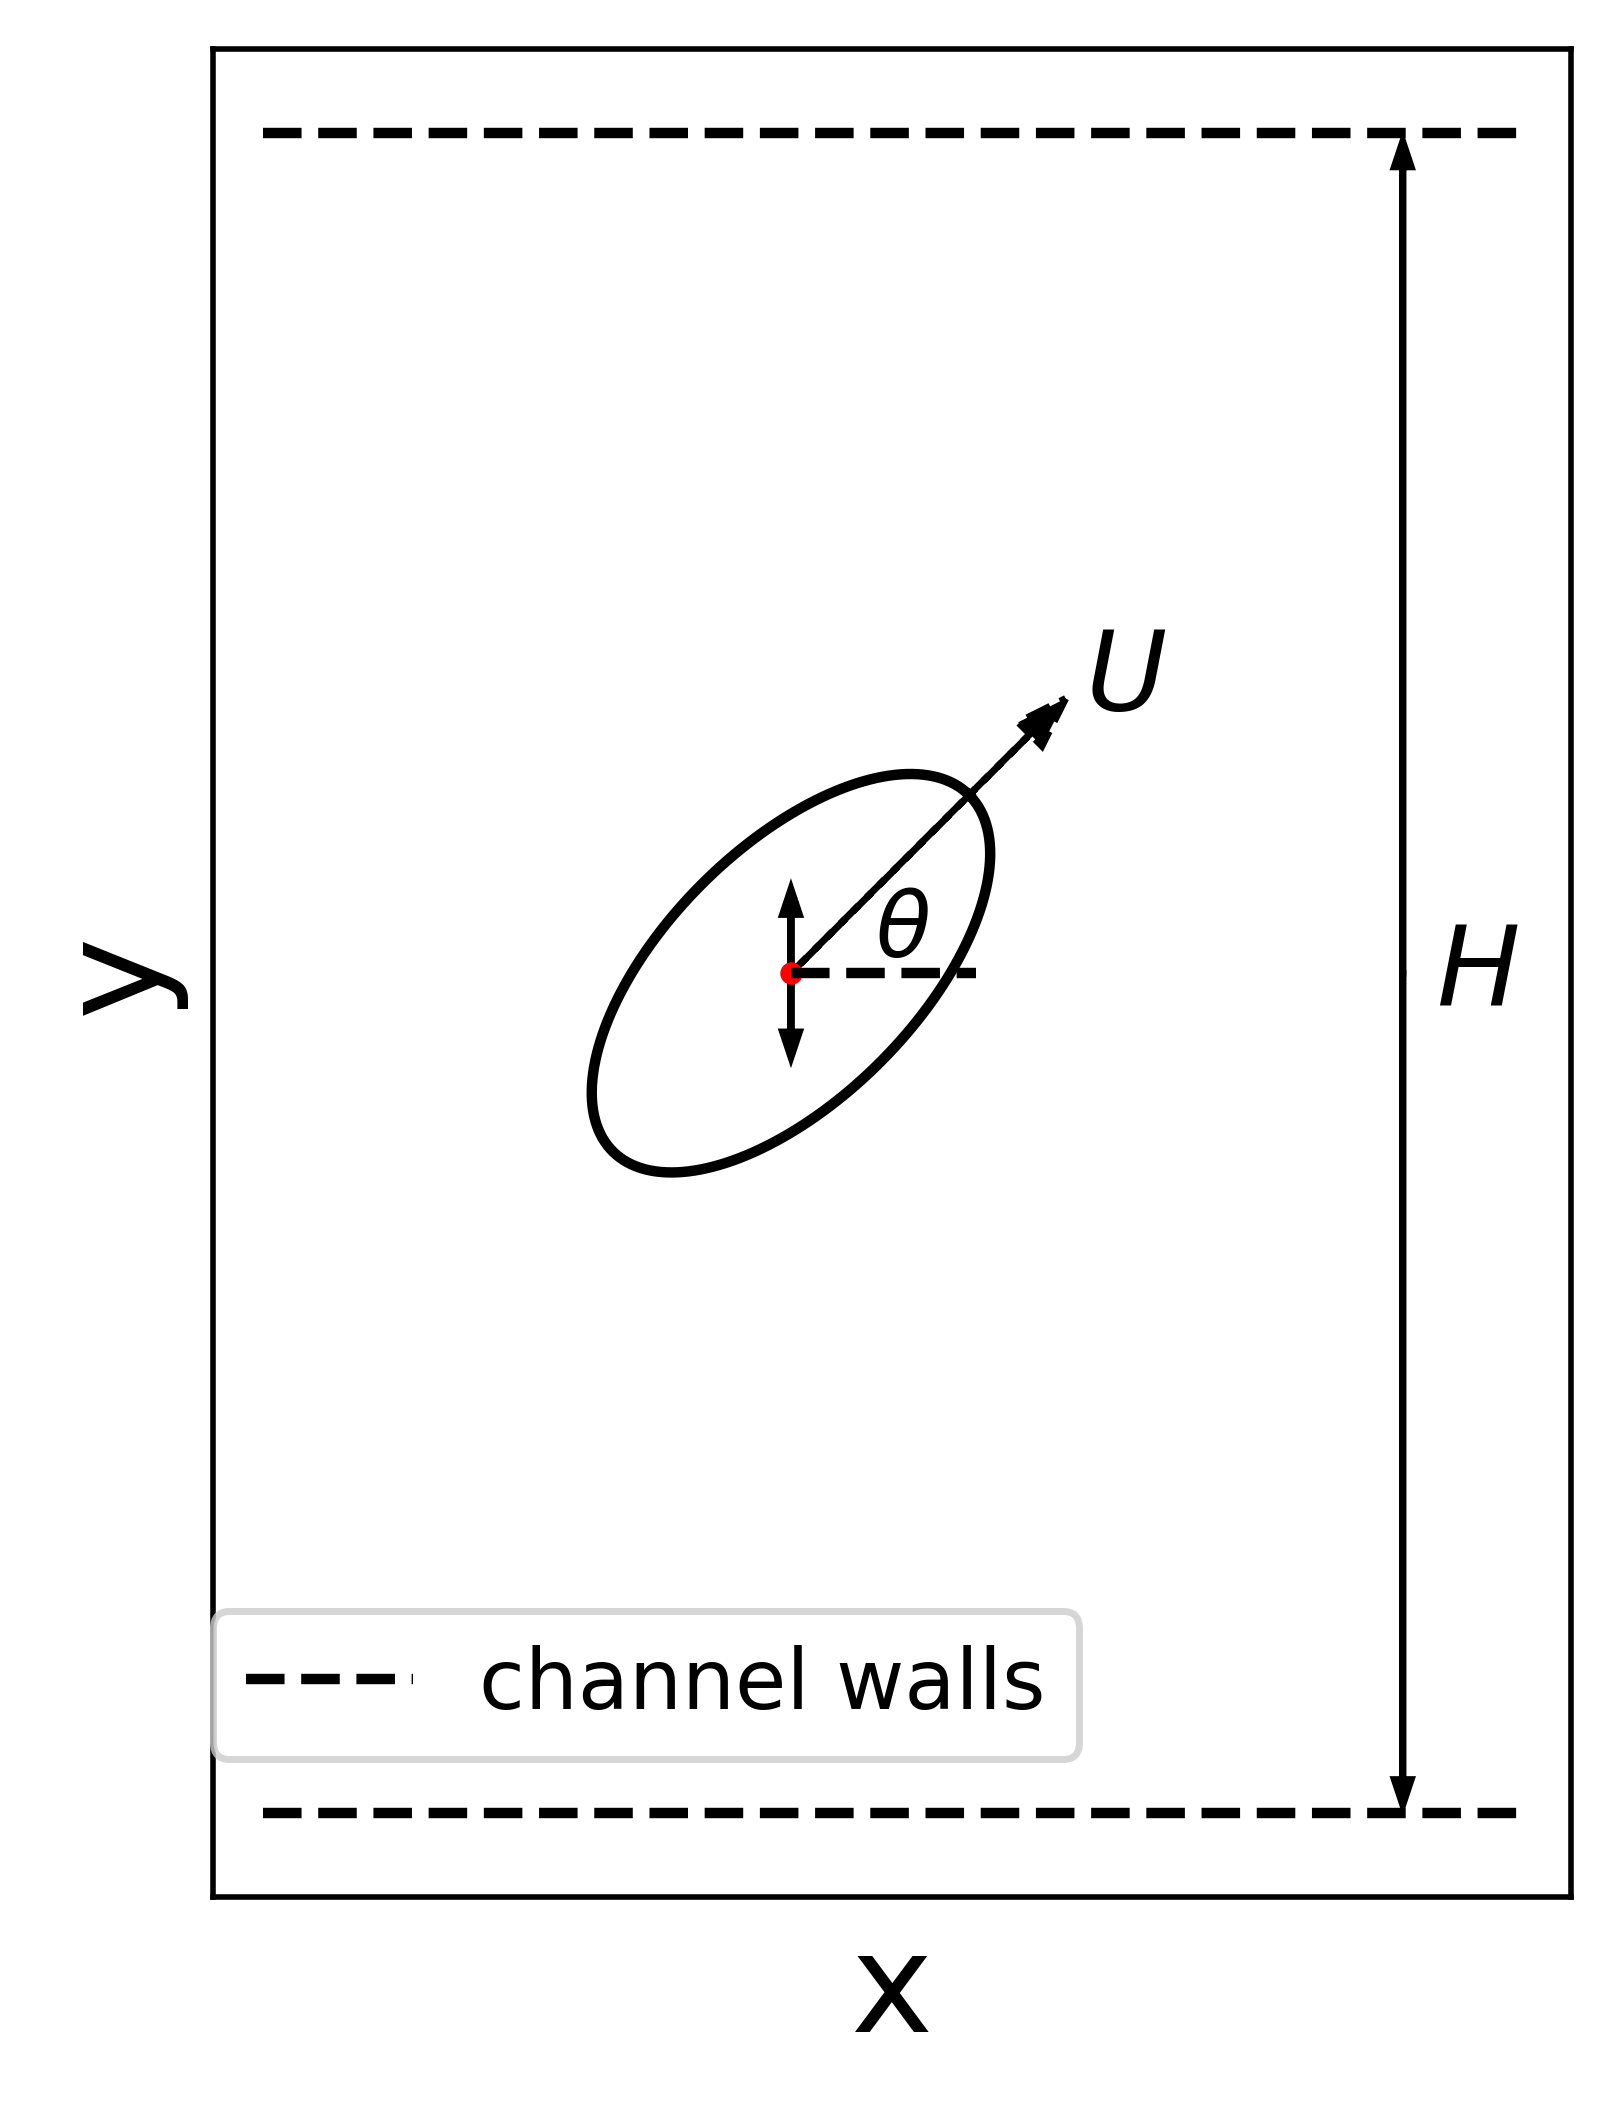
\includegraphics[scale=0.5]{graphics/model1_setup.png}
    \caption{An elliptic cell with orientation $\theta$ located within a channel of fixed height H
    and infinite width. The channel walls are considered reflective boundaries.}
    \label{fig:model1_setup}
\end{figure}

The dynamics imposed on the cell are described by the following coupled SDEs:

\begin{subequations}\label{eq:model1_sdes}
    \begin{align}
        Y(t + \Delta t) &= Y(t) + U \sin(\theta) + \sqrt{2D_y}\Delta W_1 \label{eq:model1_sdes_a} \\
        \theta(t + \Delta t) &= \theta(t) + \sqrt{2D_\theta}\Delta W_2 \label{eq:model1_sdes_b}
    \end{align}
\end{subequations}

Here, $Y(t)$ denotes the vertical position of the cell's geometric centre at time $t$,
and $\theta$ its orientation at that time. The parameters 
$D_y$ and $D_\theta$ scale the respective Brownian motion terms, modelling random
fluctuations in position and orientation. The parameter $U$ sets the deterministic speed 
of the cell's motion along the $y$-axis, thereby controlling the magnitude of the directed 
movement within the channel. We treat the upper and lower channel walls as 
reflective boundaries. Movement along the $x$-axis is disregarded, as our primary interest is in understanding
whether this system exhibits boundary accummulation behaviour. Given the channel's infinite extent along
the $x$-axis, horizontal movements have no meaningful impact on the boundary accumulation analysis. 
care primarily about whether this system exhibits boundary accummulating behaviour. With no bounds along $x$, 
it is irrelevant to consider movement along the $x$-axis. 

Our primary objective is to identify whether this system exhibits boundary accummulation behaviour. To
investigate this, we seek the stationary distribution - the long-term PDF to which the system converges as
$t \to \infty$. To obtain this stationary distribution, two approaches are available: Performing Monte Carlo 
simulations using equations \eqref{eq:model1_sdes}, or directly solving the corresponding Fokker-Planck PDE.

Both of these approaches however first require us to identify the configuration space of the system - the space of 
possible configurations of $y$ and $\theta$ the system can inhabit. As the cell's orientation $\theta$ is periodic
and thus unbounded, the vertical position $y$ is constrained by the channel walls. SPecifically, the minimum 
distance the centre of the clel can approach each channel wall depends expicitly on its orientation $\theta$. 
This dependency is illustrated in Figure \ref{fig:rolling_oval}.

\begin{figure}[htbp]
    \centering
    \includegraphics[scale=0.45]{graphics/rolling_oval.png}
    \caption{Path traced by the oval's centre, illustrating the minimum distance achievable to a horizontal
    wall as a function of orientation $\theta$}
    \label{fig:rolling_oval}
\end{figure}

The function characterising this minimum distance is termed the \textit{wall distance} function
\cite{chen2021shape}. For the specific case of an ellipse, this function is defined by:

\begin{subequations}\label{eq:wall_dist_funcs}
    \begin{align}
        y_{min}(\theta) &= \sqrt{a^2\sin^2(\theta) + b^2\cos^2(\theta)} \\
        y_{max}(\theta) &= H - \sqrt{a^2\sin^2(\theta) + b^2\cos^2(\theta)}
    \end{align}
\end{subequations}

where $a$ and $b$ are the major and minor semi-axes for the elliptic cell, respectively. 
Equations \eqref{eq:wall_dist_funcs} establish the upper and lower boundaries of the configuration space for this
system.Figure \ref{fig:configuration_space_model_1} illustrates the derived configuration space.

\begin{figure}[htbp]
    \centering
    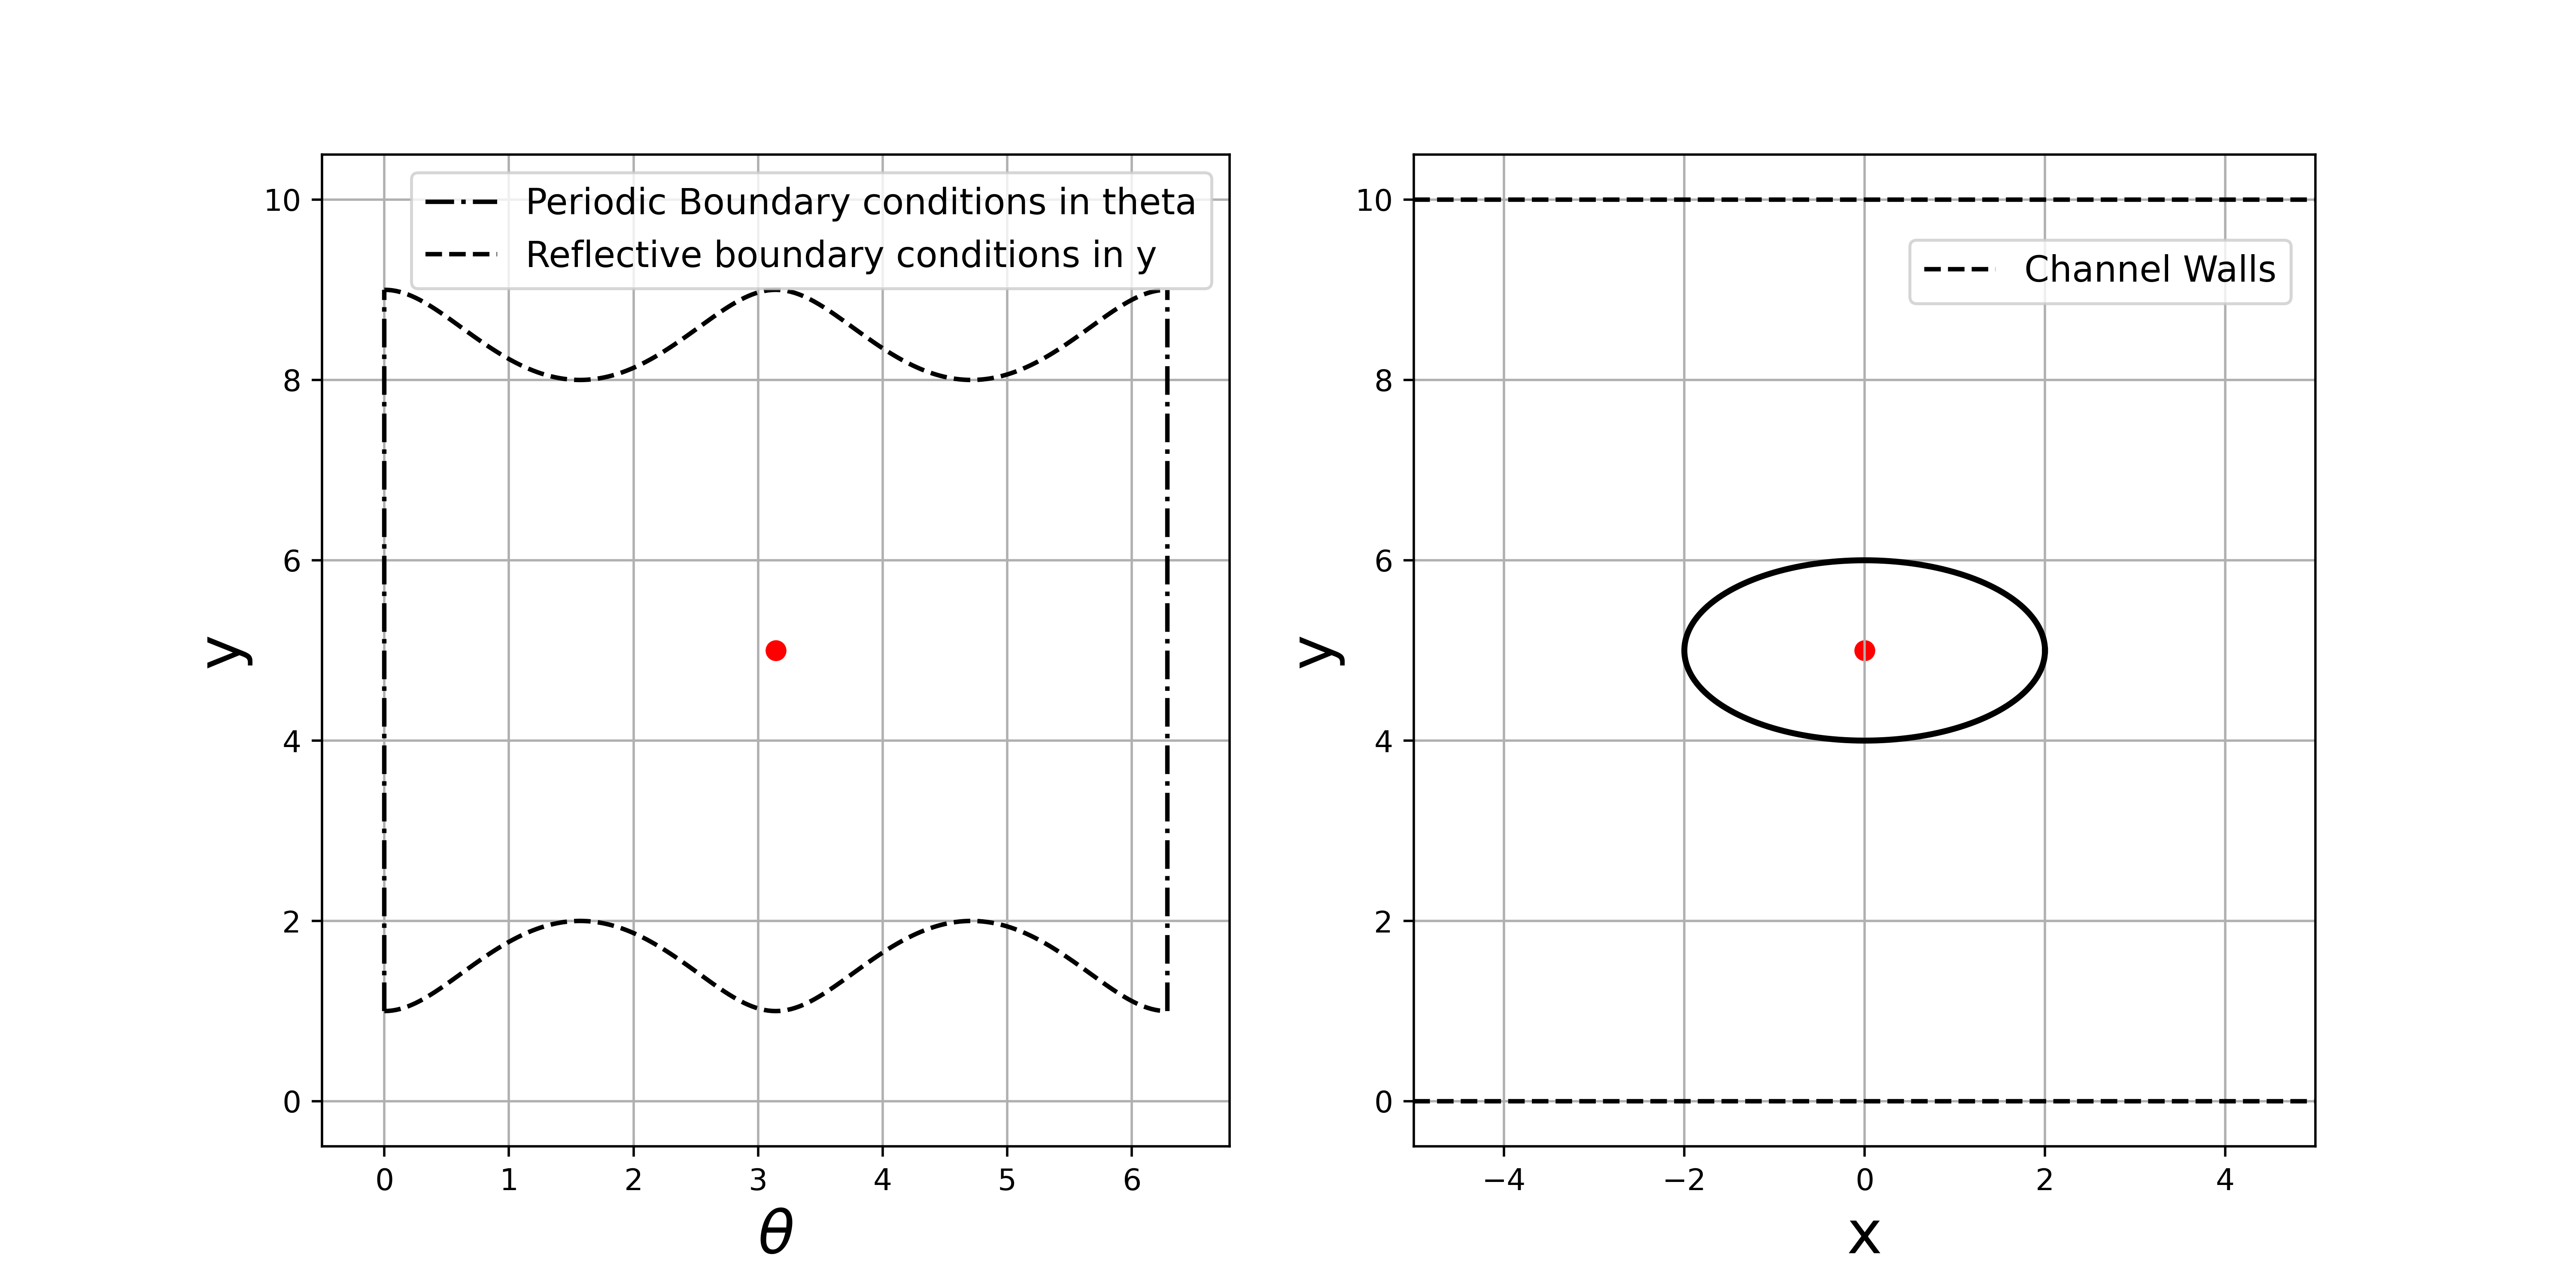
\includegraphics[scale=0.45]{graphics/config_space_1.png}
    \caption{Configuration space for Model 1 and its correspondance to 
    the physical system of a cell within a channel. Parameters used: $a=2$, $b=1$, $H=10$}
    \label{fig:configuration_space_model_1}
\end{figure}

Figure \ref{fig:configuration_space_model_1} also shows the boundary conditions 
applied to the configuration space. Periodic boundary conditions on the orientation variable
$\theta$ at $\theta=0$ and $\theta=2\pi$, while reflective boundary conditions are applied
at the upper and lower boundaries described by $y_{min}(x)$ and $y_{max}(x)$.

With a clearly bounded configuration space, the corresponding 
Fokker-Planck equation associated with equations \eqref{eq:model1_sdes} can be solved. The corresponding Fokker-Planck
equation is:

\begin{equation}\label{eq:model_1_fokker_planck}
    \frac{\partial p}{\partial t} = -\frac{\partial}{\partial y} (U\sin(\theta) p) 
    + D_{\theta} \frac{\partial^2 p}{\partial \theta^2} 
    + D_y \frac{\partial^2 p}{\partial y^2}
\end{equation}


When solving equation \eqref{eq:model_1_fokker_planck}, no-flux boundary conditions are applied at the upper and lower
boundaries along the $y$-axis, accounting for the conservation of probability within the domain. 
The finite element solver COMSOL Multiphysics\textregistered was used to numerically obtain the stationary distribution 
\cite{comsol}. The resulting PDF is presented in Figure \ref{fig:subfig_model_1_pdf}, and the resulting marginal 
distribution across the channel is displayed in Figure \ref{fig:subfig_model_1_marginal_y}.


\begin{figure}[htbp]
    \centering
    \begin{subfigure}[b]{0.45\textwidth}
        \centering
        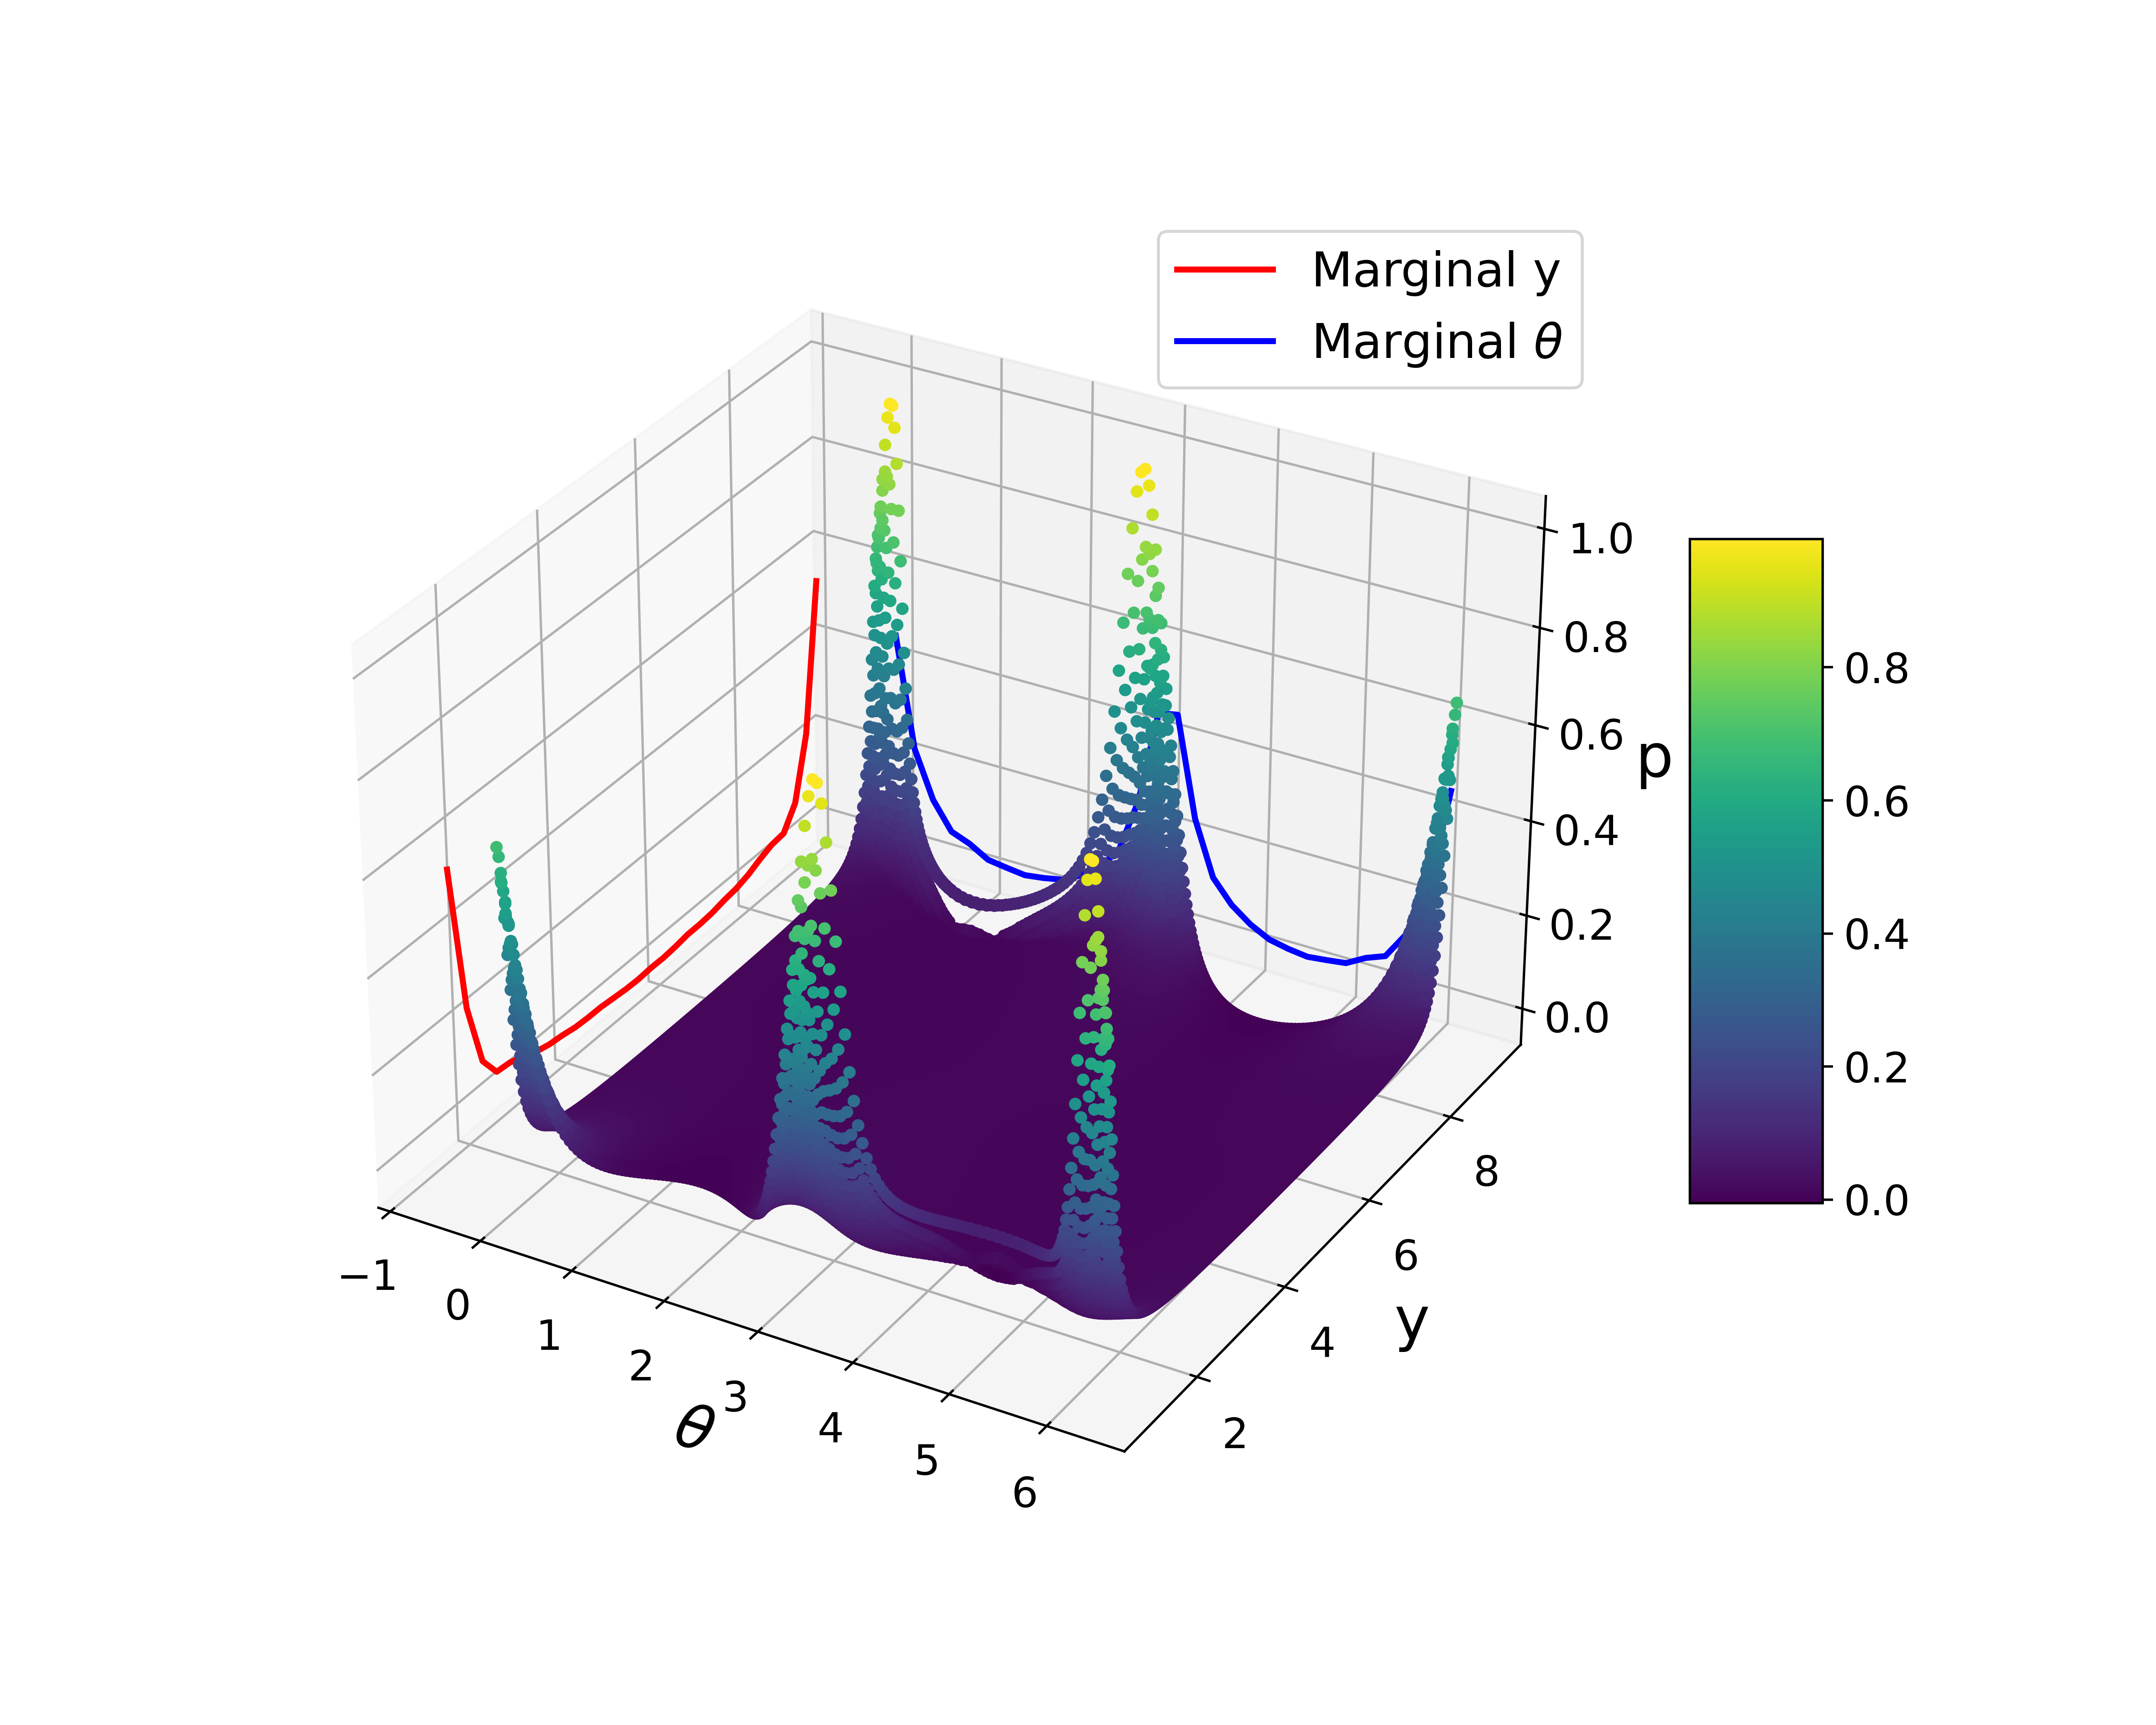
\includegraphics[width=\textwidth, trim=30 20 30 20, clip]{graphics/model_1_pdf_surface.png}
        \caption{Stationary distribution obtained for equations \eqref{eq:model1_sdes}. Marginal distributions are displayed along 
        the axes margins.}
        \label{fig:subfig_model_1_pdf}
    \end{subfigure}
    \hfill
    \begin{subfigure}[b]{0.45\textwidth}
        \centering
        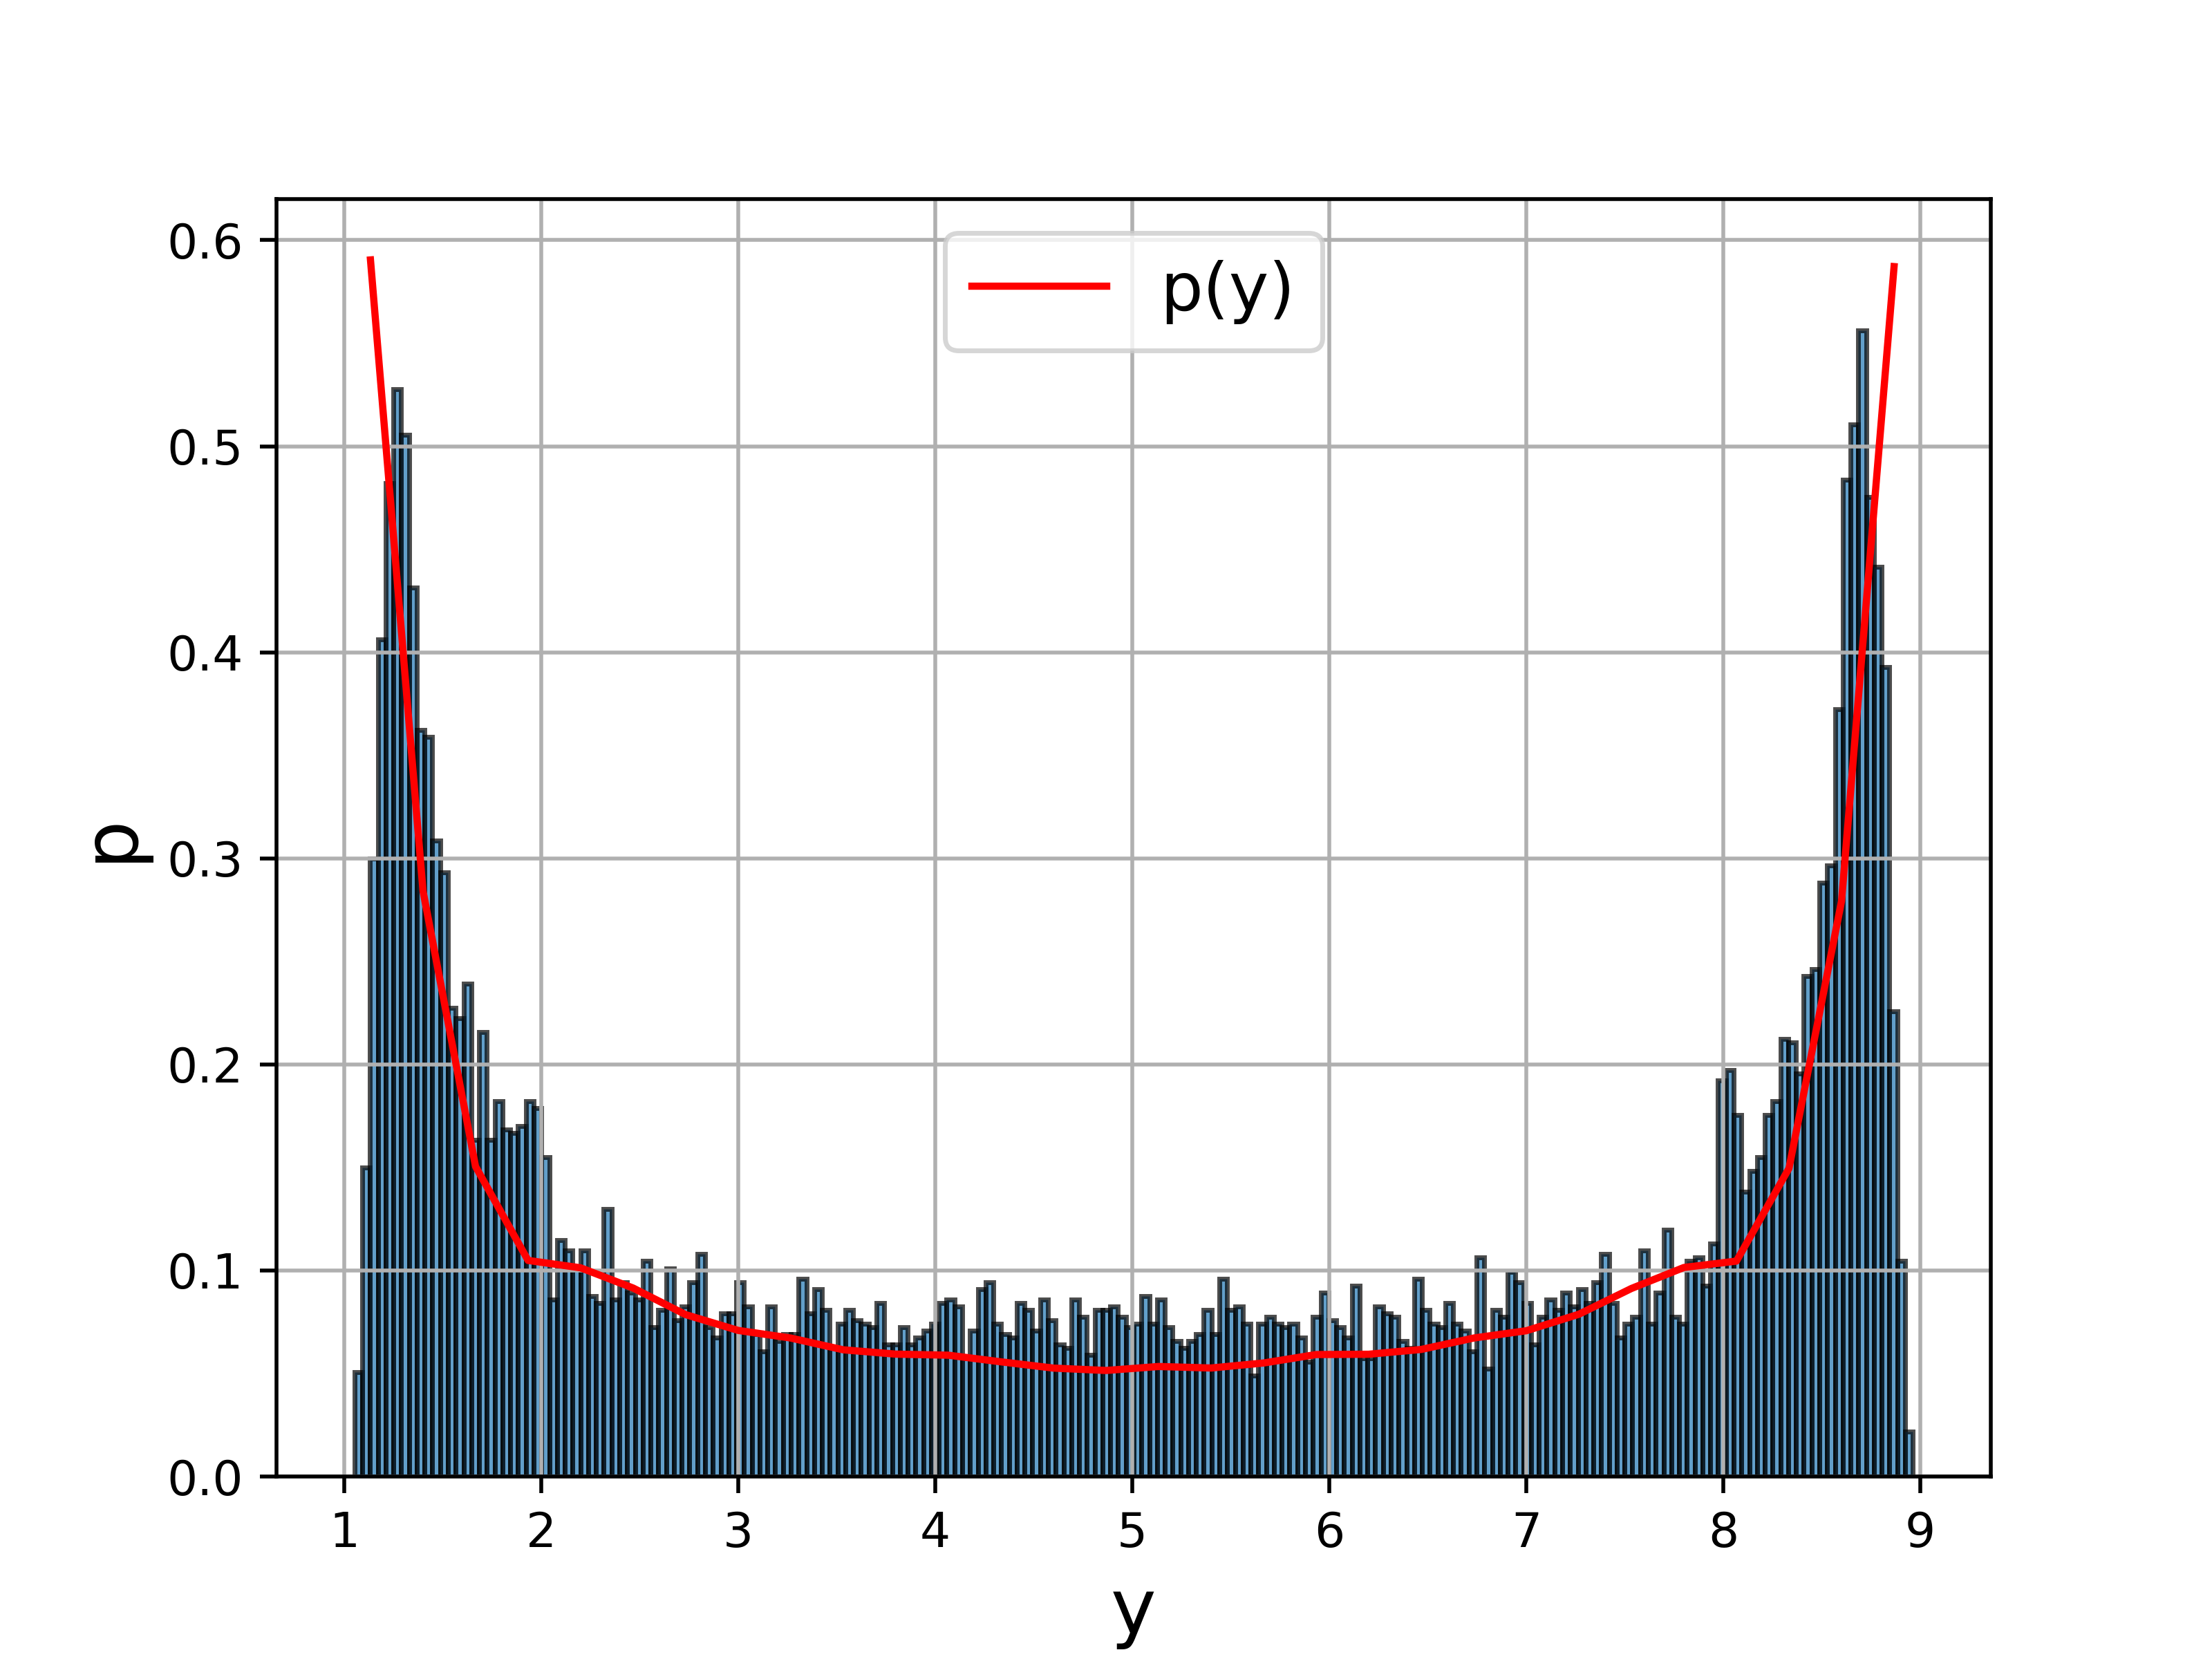
\includegraphics[width=\textwidth]{graphics/model_1_marginal_y.png}
        \caption{Marginal distributions along $y$ derived from solving the Fokker-Planck (red line) and from
         Monte Carlo simulation (histogram)}
        \label{fig:subfig_model_1_marginal_y}
    \end{subfigure}
    \caption{Comparison of stationary distribution and its marginal along $y$.}
    \label{fig:model_1_results}
\end{figure}

The marginal distribution along the $y$-axis clearly exhibits characteristic boundary accumulation behaviour. 
We attribute this phenomenon as arising from two primary mechanisms. Firstly, the drift term in equation \eqref{eq:model1_sdes_a} 
implies that, on average, the cell moves towards and eventually encounters the boundary, where it becomes constrained 
until it sufficiciently reorients. Secondly, the geometry of the configuration space contributes significantly; the elliptical
shape introduces two "hills" with reflective boundaries. These features act as barriers, hindering the ease with 
which the system can exit the boundary regions, thus enhacing the boundary accummulation.

\subsection{Model 2: Hydrodynamics Informed Model}\label{sec:hydrodynamic_model}
The second modelinvestigated was proposed by Chen \textit{et al}. \cite{chen2021shape}, 
building on the work of Spagnolie \textit{et al}. 
\cite{spagnolie2015geometric}. This advances  on the previous model by incorporating hydrodynamic interactions
with the channel walls into the SDEs for the cell.

Spagnolie \textit{et al.} approximate the velocity field around an elliptic swimmer by first treating the system as a 
\textit{stresslet} - a force dipole - and then by Faxén's Law obtaining the corresponding velocity field for a 
swimmer with elliptic shape. Figure shows two illustrative charts of a microswimmer treated as a stresslet, and the 
velocity field around this elliptic stresslet near the boundary. 

\begin{figure}[htbp]
    \centering
    \begin{subfigure}[b]{0.45\textwidth}
        \centering
        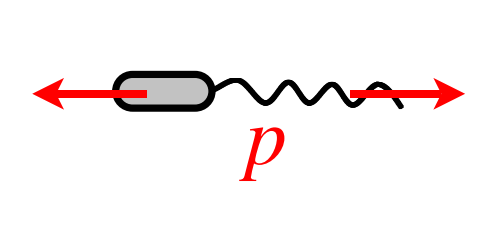
\includegraphics[width=\textwidth]{graphics/pusher_pic.png}
        \caption{Stationary}
        \label{fig:pusher_chart}
    \end{subfigure}
    \hfill
    \begin{subfigure}[b]{0.45\textwidth}
        \centering
        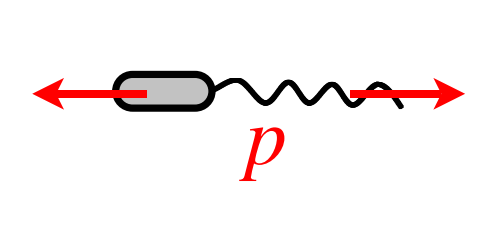
\includegraphics[width=\textwidth]{graphics/pusher_pic.png}
        \caption{Marginal}
        \label{fig:fluid_field_pusher}
    \end{subfigure}
    \caption{Comparison of stationary distribution and its marginal along $y$.}
    \label{fig:model_2_intro}
\end{figure}

% It is worth noting that in the literature microswimmers are categorised as either 
% \textit{pushers} 

\subsection{Model 3: Bulk and Boundary Model}\label{sec:bulk_and_boundary_model}
The third model considered is proposed by Fu et al. \cite{fu2021fokker}. They
propose a simplified model that expliclty incorporates boundary accummulation. Stochasticity is
only present in the angular variable $\theta$, and there is no shape or hydrodynamic 
forces incorporated, so only a point particle is considered.

The model imposes boundary accumulation by introducing a free-swimming phase (FSP) and two boundary
capture phases, corresponding to interactions with the upper and lower channel walls. In the 
free-swimming phase, the cell swims at a constant speed $U$ while experiencing stochasticity solely
in its angular orientation. Upon contact with either boundary, the cell transitions to a 
boundary-capture phase (BCP), remaining stationary at the boundary until its orientation changes
sufficiently - due to continued rotational Brownian motion - to direct its trajectory away from
the wall. 

The SDEs describing this system are:

\begin{subequations}\label{eq:model_3_sdes}
    \begin{align}
        Y(t + \Delta t) &=
        \begin{cases}
            Y(t) + U \sin(\theta) \Delta t, & \text{if } |Y(t)| \le \frac{H}{2} \text{or } 
            |Y(t)| = \frac{H}{2} \text{and } Y(t) \theta(t) \leq 0 \\
            Y(t), & \text{if } |Y(t)| = \frac{H}{2} \text{and } Y(t) \theta(t) \ge 0
        \end{cases} \\
        \theta(t + \Delta t) &= \theta(t) + \sqrt{2D_{\theta}}dW.
    \end{align}
\end{subequations}

In this model, the vertical coordinate system is centred such that $y=0$ corresponds to the 
midpoint of the chanel, with channel boundaries positioned at $y=\frac{H}{2}$ and 
$y = -\frac{H}{2}$. Additionally, $\theta$ now ranges between $[-\pi, \pi]$. This choice
of coordinates simplifies the conditional statements in equations \eqref{eq:model_3_sdes}.
An illustration of the model is shown in Figure \ref{fig:model_3_setup}. 

\begin{figure}[htbp]
    \centering
    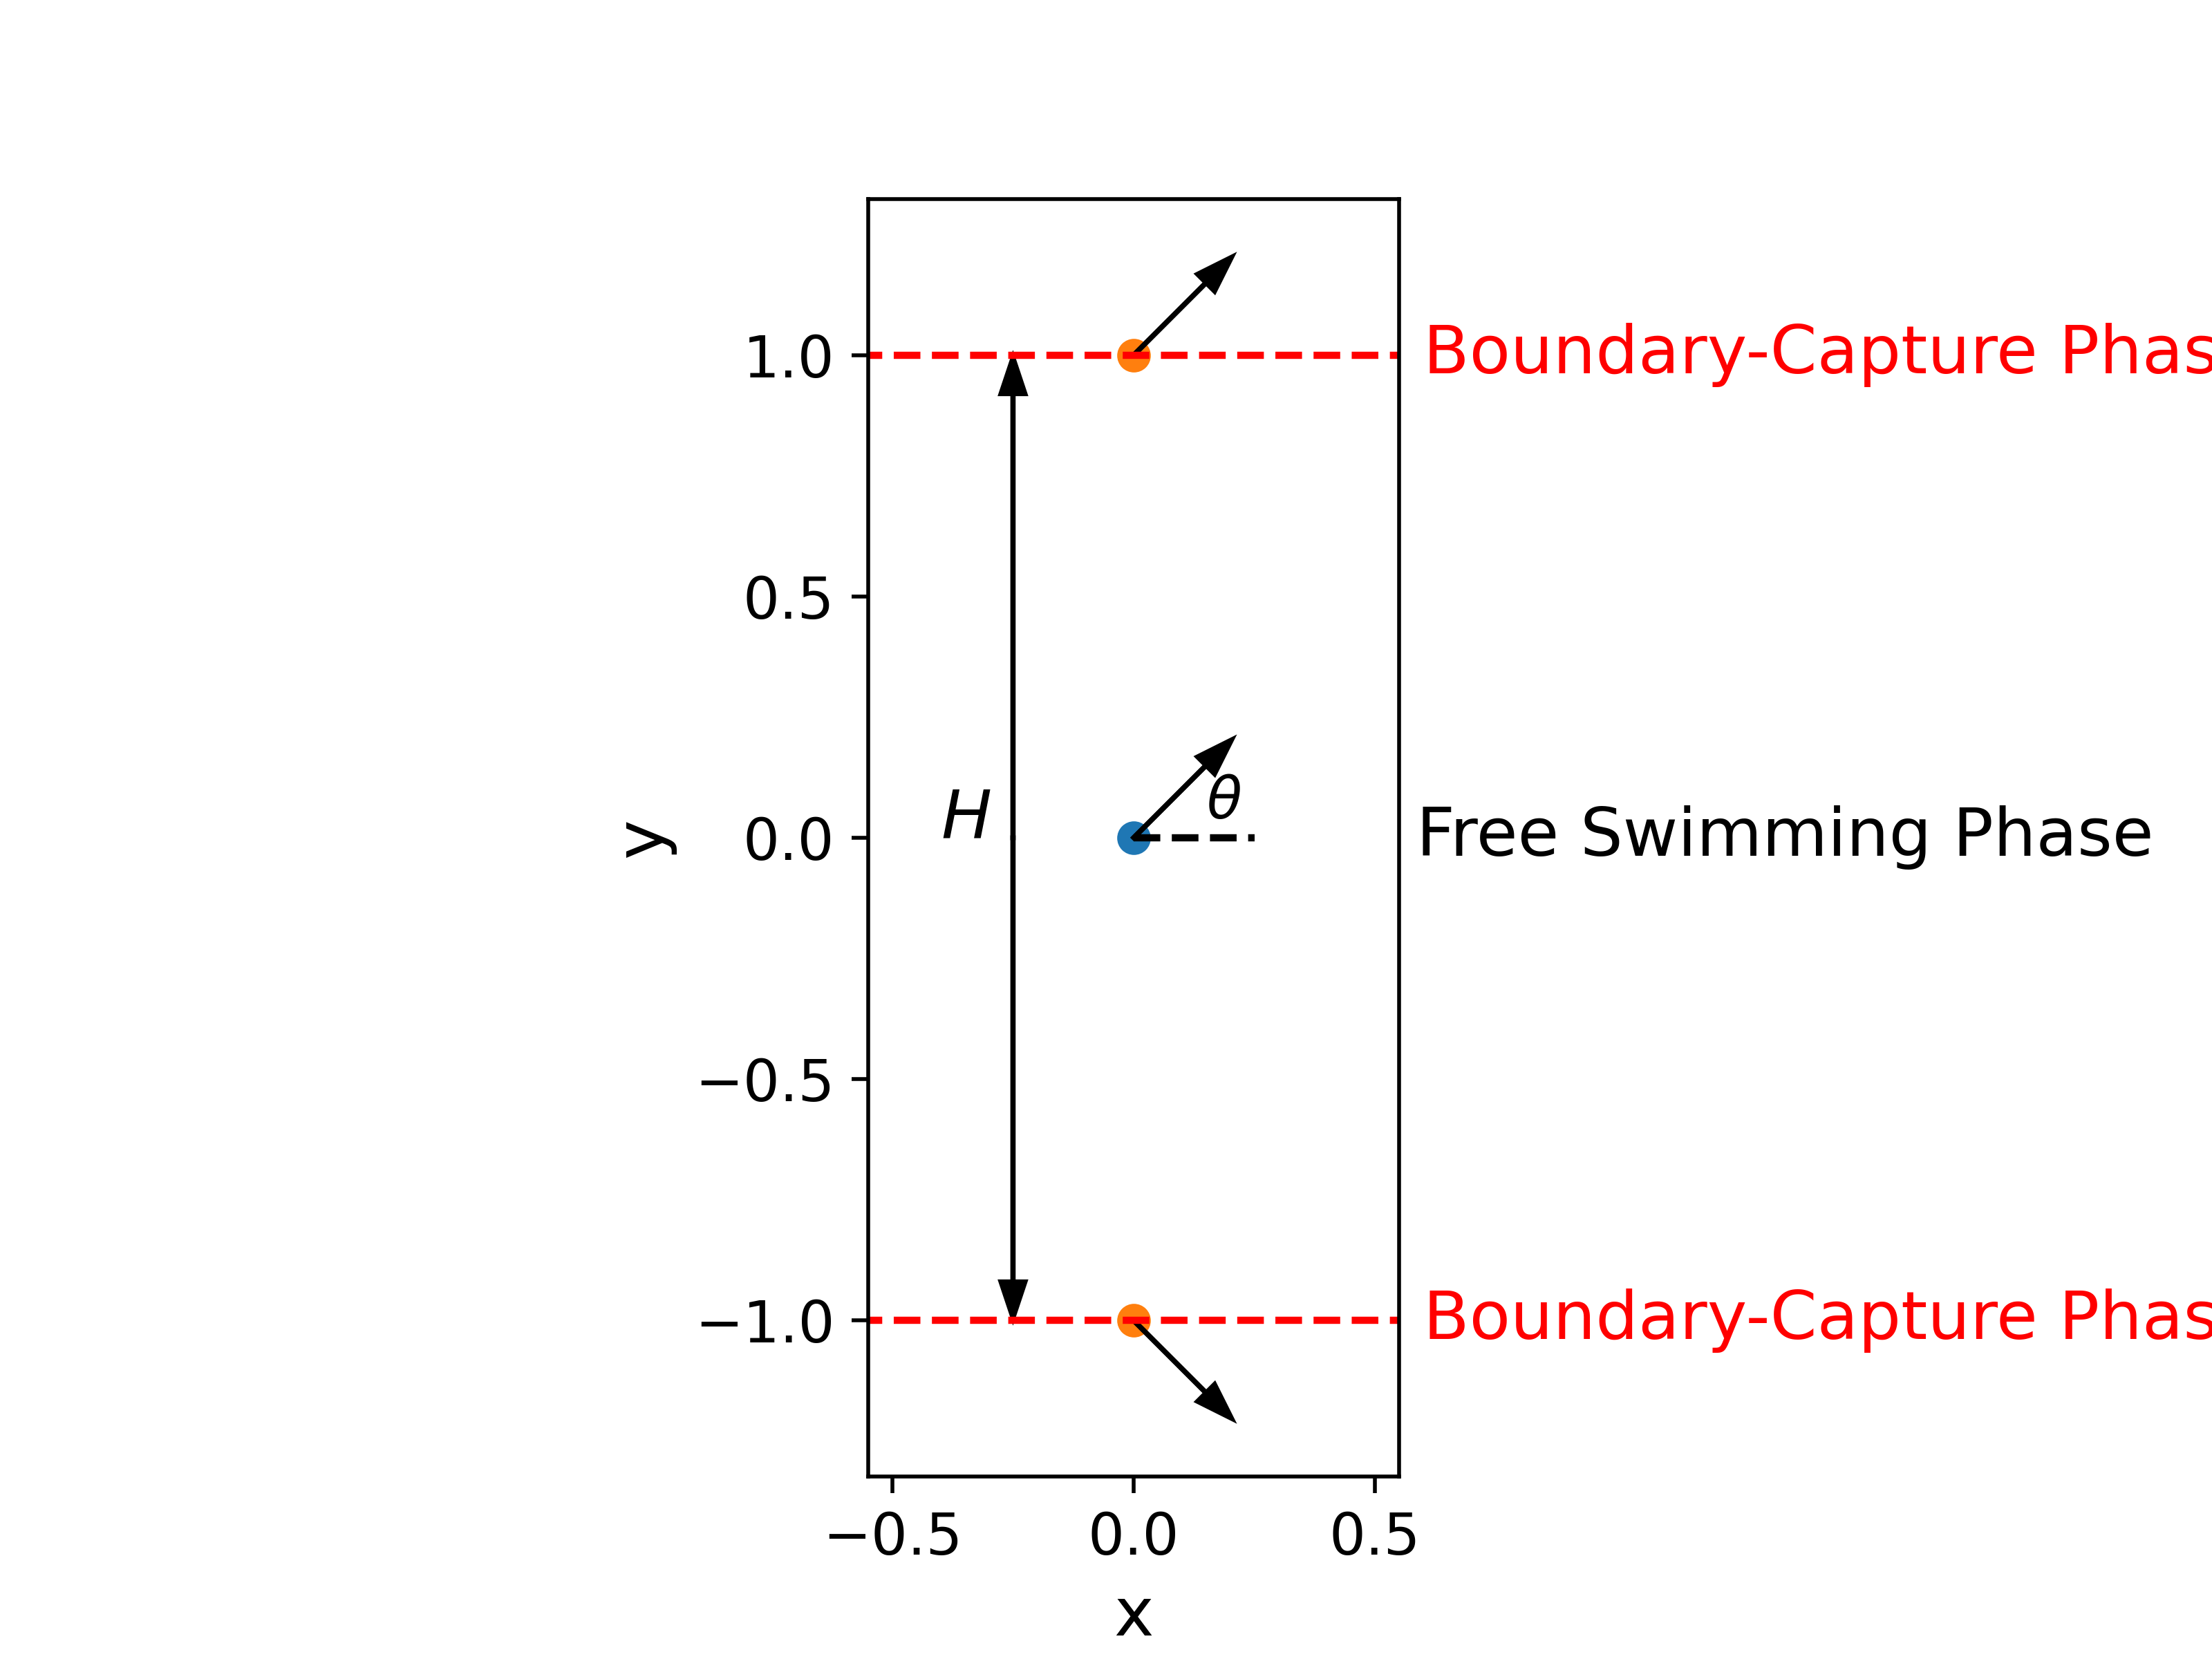
\includegraphics[scale=0.5]{graphics/model_3_setup.png}
    \caption{Schematic illustration of the system configuration for Model 3. Microswimmer is 
    treated as a point particle in a channel of height $H=2$, with boundaries at
    $y=\frac{H}{2}$ and $y=-\frac{H}{2}$. The particle remains trapped at a boundary until 
    its orientation is redirected inward, away from the boundary.}
    \label{fig:model_3_setup}
\end{figure}

The authors propose the following Fokker-Planck system for SDEs \eqref{eq:model_3_sdes}. 
These equations are degenerate, as the particles motion in $y$ is deterministic.

\begin{subequations}\label{eq:model_3_fk}
    \begin{align}
        & \frac{\partial p}{\partial t} + U \sin(\theta) \frac{\partial p}{\partial y} - D_\theta \frac{\partial^2 p}{\partial \theta^2}, \quad (y, \theta) \in \Omega \label{eq:fsp_sde} \\
        & \frac{\partial p_+}{\partial t} - D_\theta \frac{\partial^2 p_+}{\partial \theta^2} = U \sin(\theta)p(t, \frac{H}{2}, \theta), \quad (\frac{H}{2}, \theta), \quad (\frac{H}{2}, \theta) \in \Omega_+ \label{eq:bcp_sde_up}\\
        & \frac{\partial p_-}{\partial t} - D_\theta \frac{\partial^2 p_+}{\partial \theta^2} = -U \sin(\theta)p(t, -\frac{H}{2}, \theta), \quad (\frac{H}{2}, \theta), \quad (-\frac{H}{2}, \theta) \in \Omega_+ \label{eq:bcp_sde_down}
    \end{align}
\end{subequations}

where $p(t, y, \theta)$ is the PDF of the cells in the FSP at time $t$, position $y$ with orientation $\theta$, while
 $p_\pm$ are the PDFs 
of boundary contacting cells at time $t$, position $\pm \frac{H}{2}$ with non-inward facing orientation. $\Omega$ 
denotes the domain occupied by cells in FSP, while $\Omega_\pm$is the domains of the 
upper and lower BCPs, respectively. 

The associated boundary conditions for \eqref{eq:model_3_fk} are as follows. First we consider the boundary
conditions associated with cells in the FSP \eqref{eq:fsp_sde}. As 
cells with direction $\theta = \pi$ and $\theta = -\pi$ are the same, we have periodic boundary 
conditions in $\theta$:

\begin{equation}
    p(t, y, -\pi) = p(t, y, \pi), \qquad \frac{\partial p}{\partial \theta}(t, y, -\pi) = \frac{\partial p}{\partial \theta},  \qquad -\frac{H}{2} < y < \frac{H}{2}
\end{equation}

Further, as it is impossible for cells in the BCP with outward-facing orientation to enter 
the FSP, we impose Dirichlet boundary conditions at the channel walls:

\begin{equation}
    p(t, L, \theta) = 0, \quad \theta \in (-\pi, 0), \qquad p(t, -L, \theta) = 0, \quad \theta \in (0, \pi).
\end{equation}

For cells in the BCP described by \eqref{eq:bcp_sde_up}, \eqref{eq:bcp_sde_down}, the cells exit this phase once
their orientation points inward, resulting in Dirichlet boundaries in BCP at
$\theta = 0$, $\theta = \pm \pi$:

\begin{equation}
    p_+(t, 0) = p_+(t, \pi) = 0, \qquad p_-(t, 0) = p_-(t, -\pi) = 0.
\end{equation}

Transitions between phases are characterised by source and sink terms, which represent probability 
fluxes between the BCP and FSP. These fluxes are described by the following conditions:

\begin{subequations}
    \begin{align}
        \frac{\partial p}{\partial \theta}(t, y, \theta)\Bigr|_{\theta=\pi_-}^{\theta = \pi_+} = 
        \frac{\partial p_+}{\partial \theta}(t, \pi_-)\delta_{y = \frac{H}{2}} 
        - \frac{\partial p_-}{\partial \theta}(t, \pi_+)\delta_{y=-\frac{H}{2}}\\
        \frac{\partial p}{\partial \theta}(t, y, \theta)\Bigr|_{\theta=0_-}^{\theta = 0_+} = 
        -\frac{\partial p_+}{\partial \theta}(t, 0_+)\delta_{y = \frac{H}{2}} 
        + \frac{\partial p_-}{\partial \theta}(t, 0_-)\delta_{y=-\frac{H}{2}}
    \end{align}
\end{subequations}

The convergece of this system is analysed by Fu et al. \cite{fu2021fokker}, and solved 
via a finite difference scheme on a stencil depicted in Figure \ref{fig:model_3_stencil}.

\begin{figure}[htbp]
    \centering
    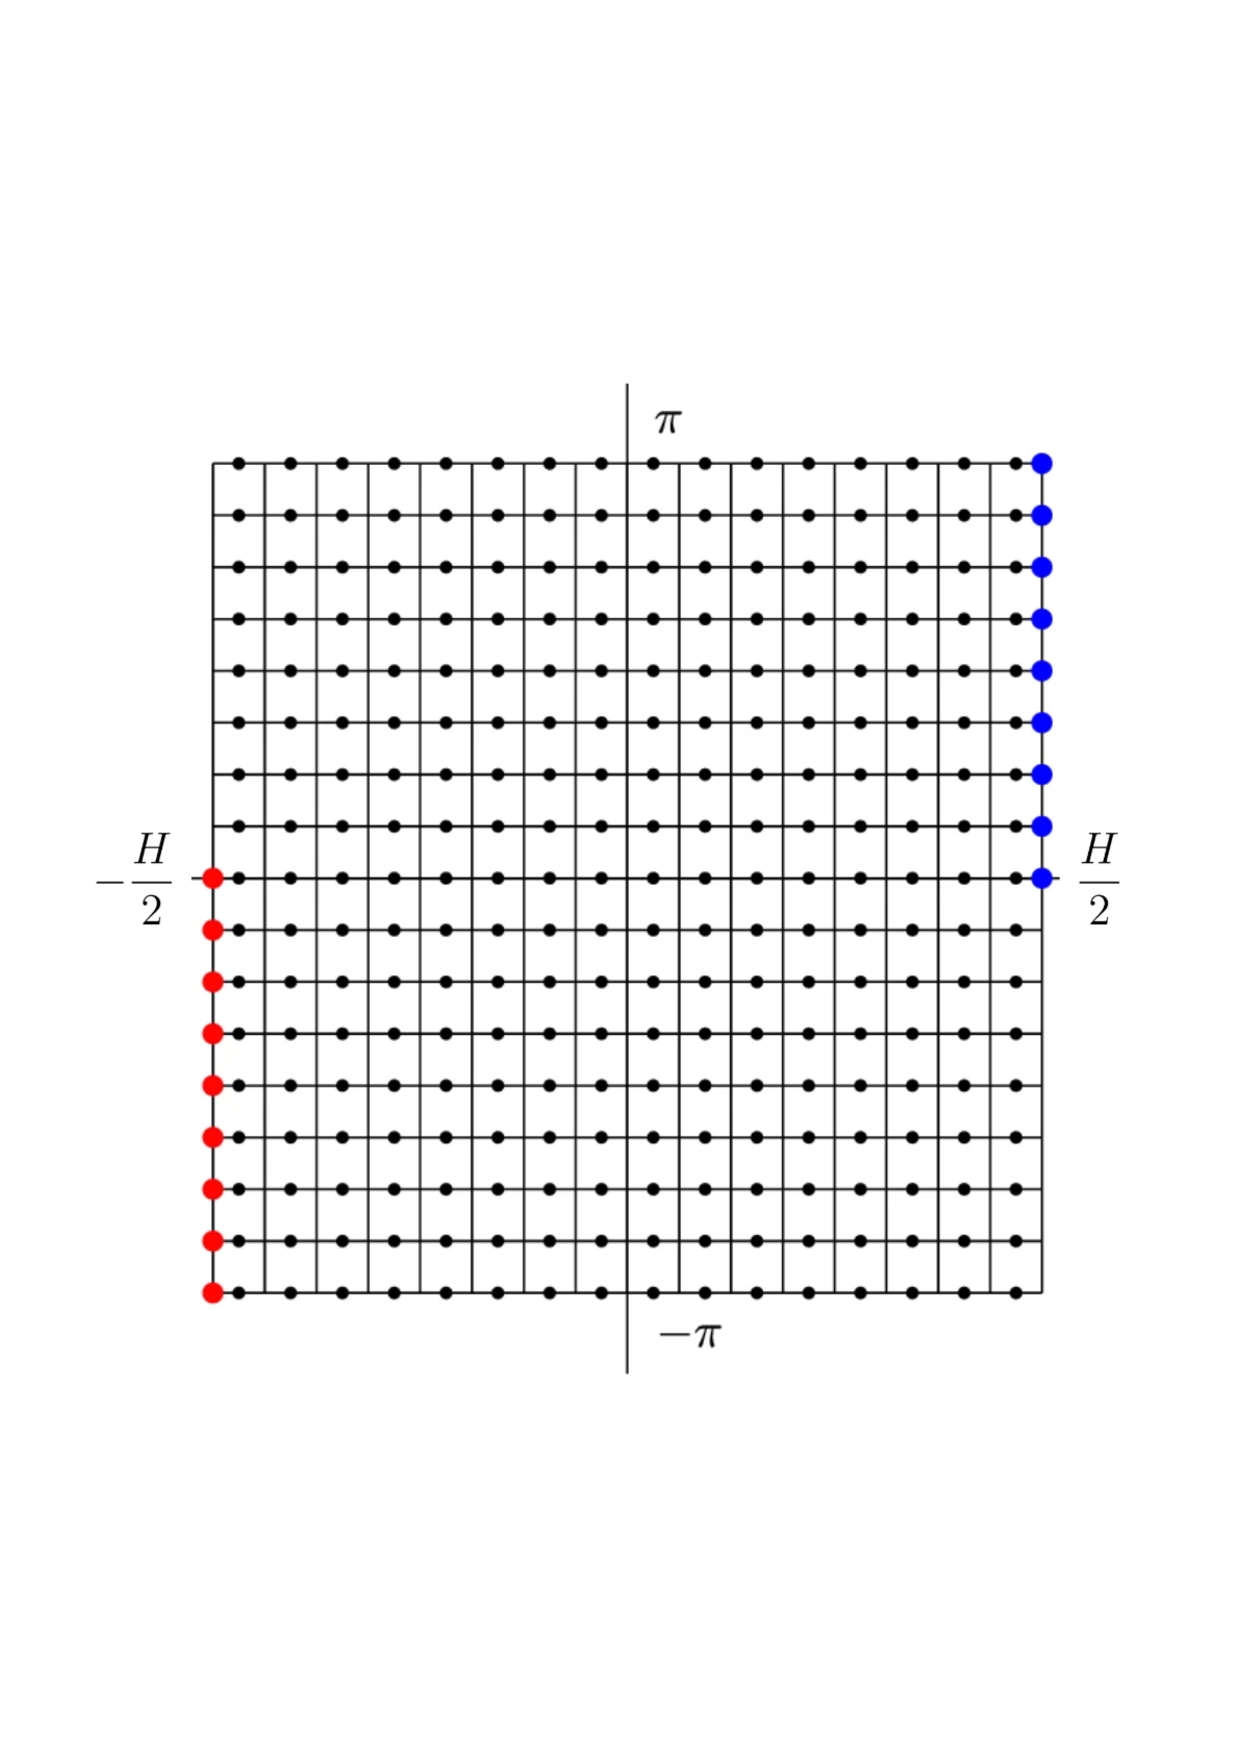
\includegraphics[scale=0.4]{graphics/model_3_stencil.pdf}
    \caption{Stencil of finite difference scheme implemented to obtain stationary distribution for \eqref{eq:model_3_fk}.
    Red dots correspond to nodes in the lower BCP, blue dots correspond to nodes in the upper BCP.}
    \label{fig:model_3_stencil}
\end{figure}


We employed both the finite-difference scheme and Monte Carlo simulations to obtain the stationary distribution 
corresopnding to equations \eqref{eq:model_3_fk}. The resulting PDF and marginal distribution is presented in 
\ref{fig:model_3_results}.

\begin{figure}[htbp]
    \centering
    \begin{subfigure}[b]{0.45\textwidth}
        \centering
        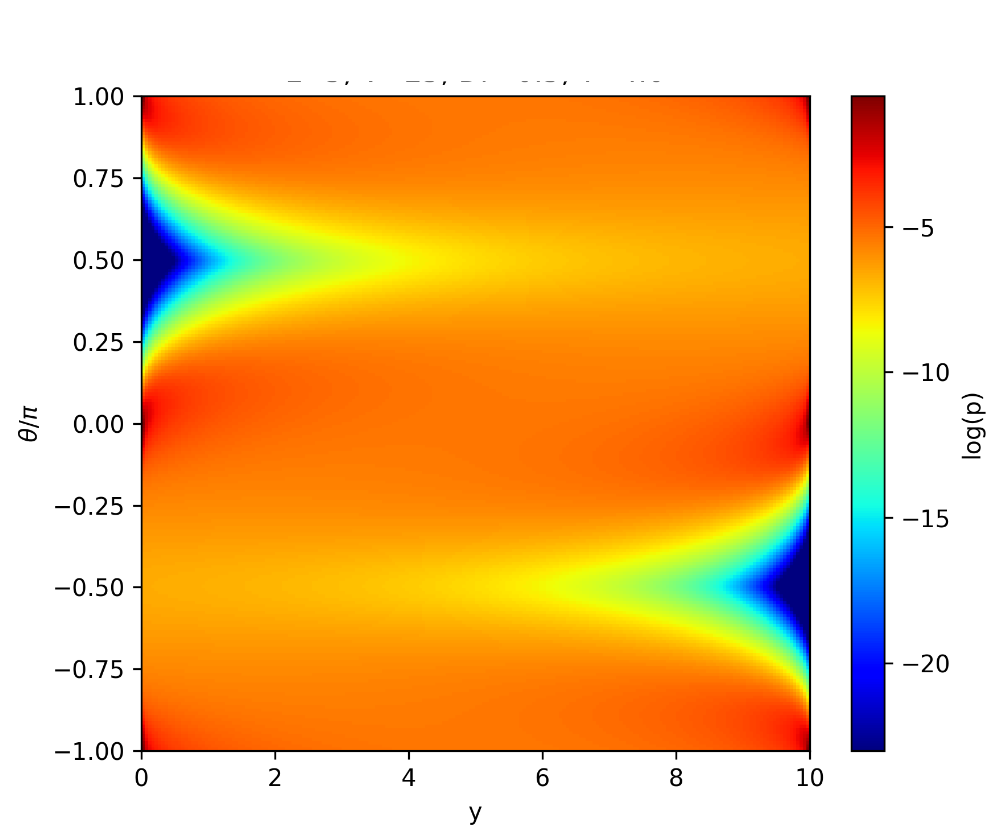
\includegraphics[scale=0.2]{graphics/model_3_pdf.png}
        \caption{Heatmap of stationary distribution obtained from \eqref{eq:model_3_fk}. 
        Parameters are: $H=10$, $U=25$, $D_\theta$=0.5.}
        \label{fig:model_3_pdf}
    \end{subfigure}
    \hfill
    \begin{subfigure}[b]{0.45\textwidth}
        \centering
        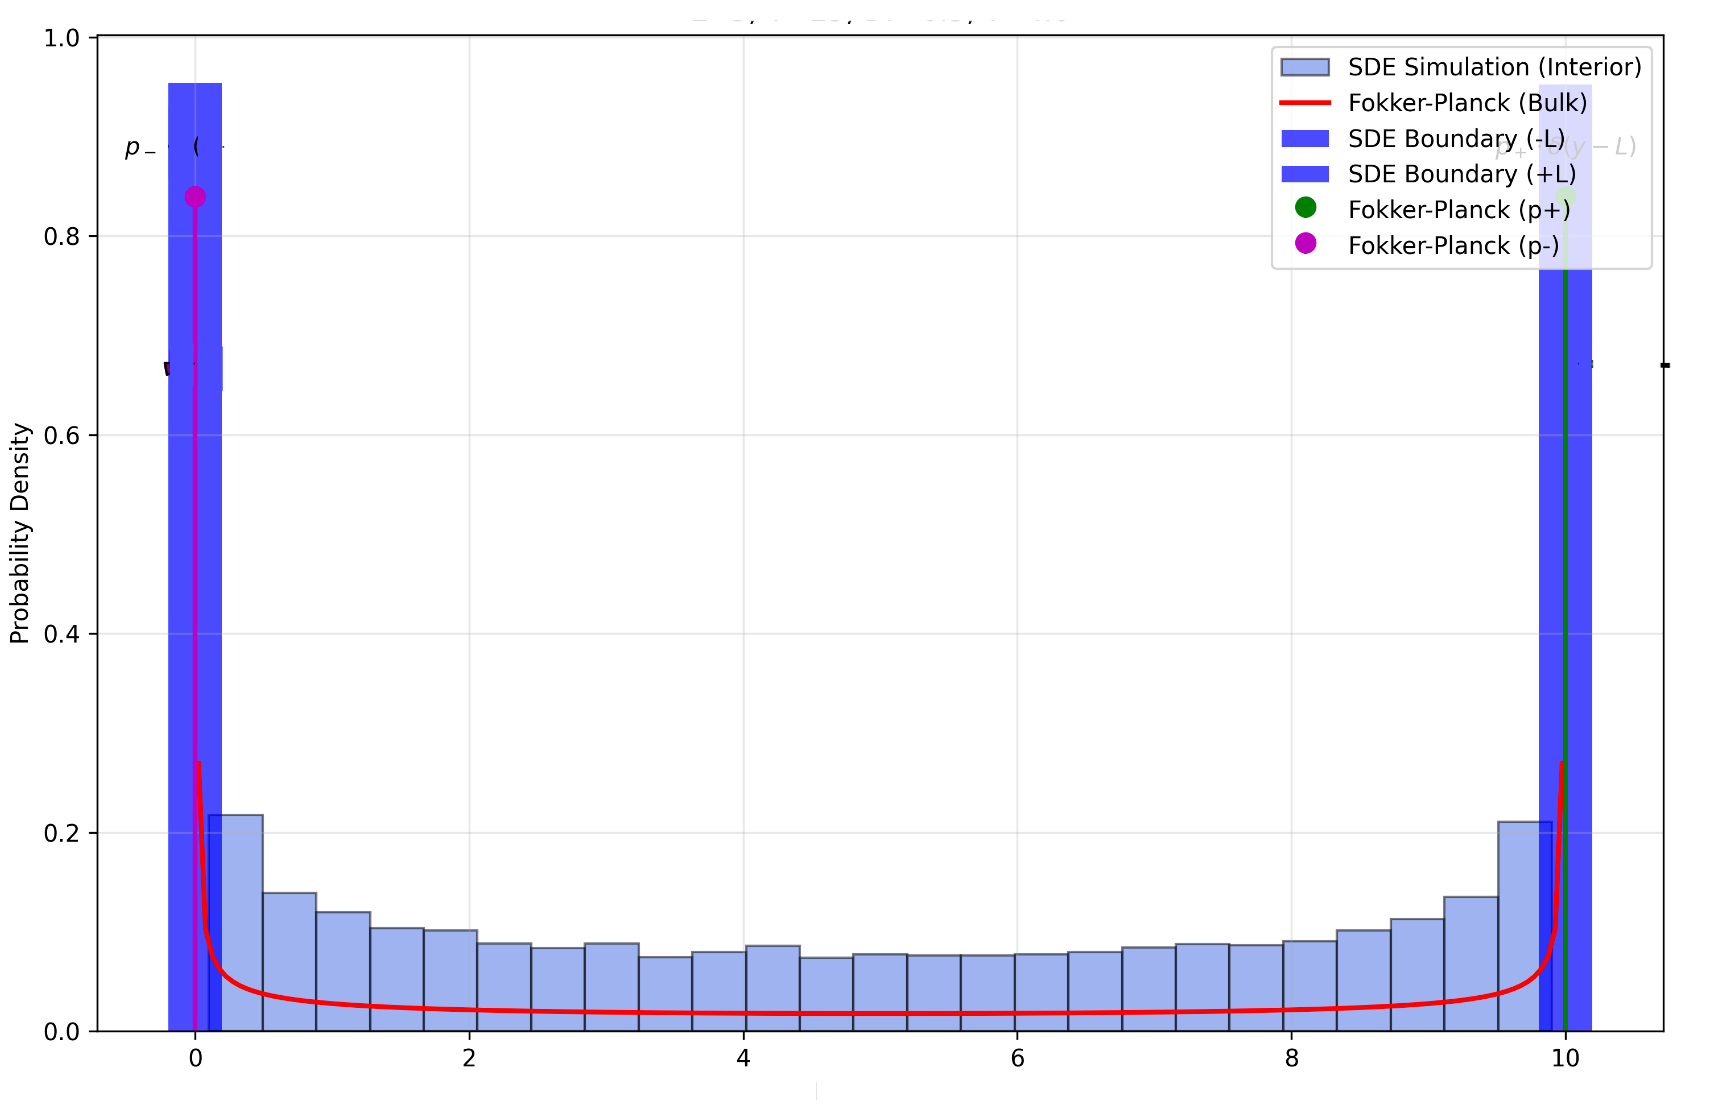
\includegraphics[width=\textwidth]{graphics/model_3_hist.png}
        \caption{Marginal distribution along the channel obtained by Monte Carlo (histogram) and 
        finite-difference scheme (solid lines).}
        \label{fig:model_3_hist}
    \end{subfigure}
    \caption{Stationary and marginal distributions for the system described by equations~\eqref{eq:model_3_fk}.}
    \label{fig:model_3_results}
\end{figure}

Figure \ref{fig:model_3_hist} demonstrates the characteristic boundary accumulation, which is expected 
given that boundary accumulation isexplicitly built into this model. Additionally, Figure \ref{fig:model_3_pdf} 
exhibits regions of extremely low probability density in the upper-left and lower-right corners. These correspond 
to regions where the cell's motion is directed opposite to its vertical orientation, making such configurations 
highly unlikely. The probability is $0$ in these regions directly against the boundary, as it is impossible for 
the cell to exit the BCP while its orrientation is against the opposite channel.





\subsection{Modifying Model 3 \& Comparison of Models}
In Model 3, the cell was treated as a point particle, neglecting the effects of cell shape on boundary interactions. 
To address this limitation, we explored incorporating cell geometry explicitly into Model 3, aiming to understand how the 
resulting PDF would compare to the shape0-dependent outcomes observed in Models 1 and 2.

This integration of shape could be implemented through multiple approaches. Our chosen method involved redistribution 
the probability mass from the boundary accumulation peaks observed in the marginal distirbution along $y$ (see Figure 
\ref{fig:model_3_hist}) over a finite region corresponding to the physical contact of an elliptical cell with the 
channel walls. Specifically, we computed the geometric average distance of an elliptically shaped cell from the 
wall and redistributed the probability previously representing 
point-particle capture in Model 3, were distirbuted. The computed average boundary distance for an ellipse is
illustrated by the solid red line in Figure \ref{fig:average_boundary}.

\begin{figure}[htbp]
    \centering
    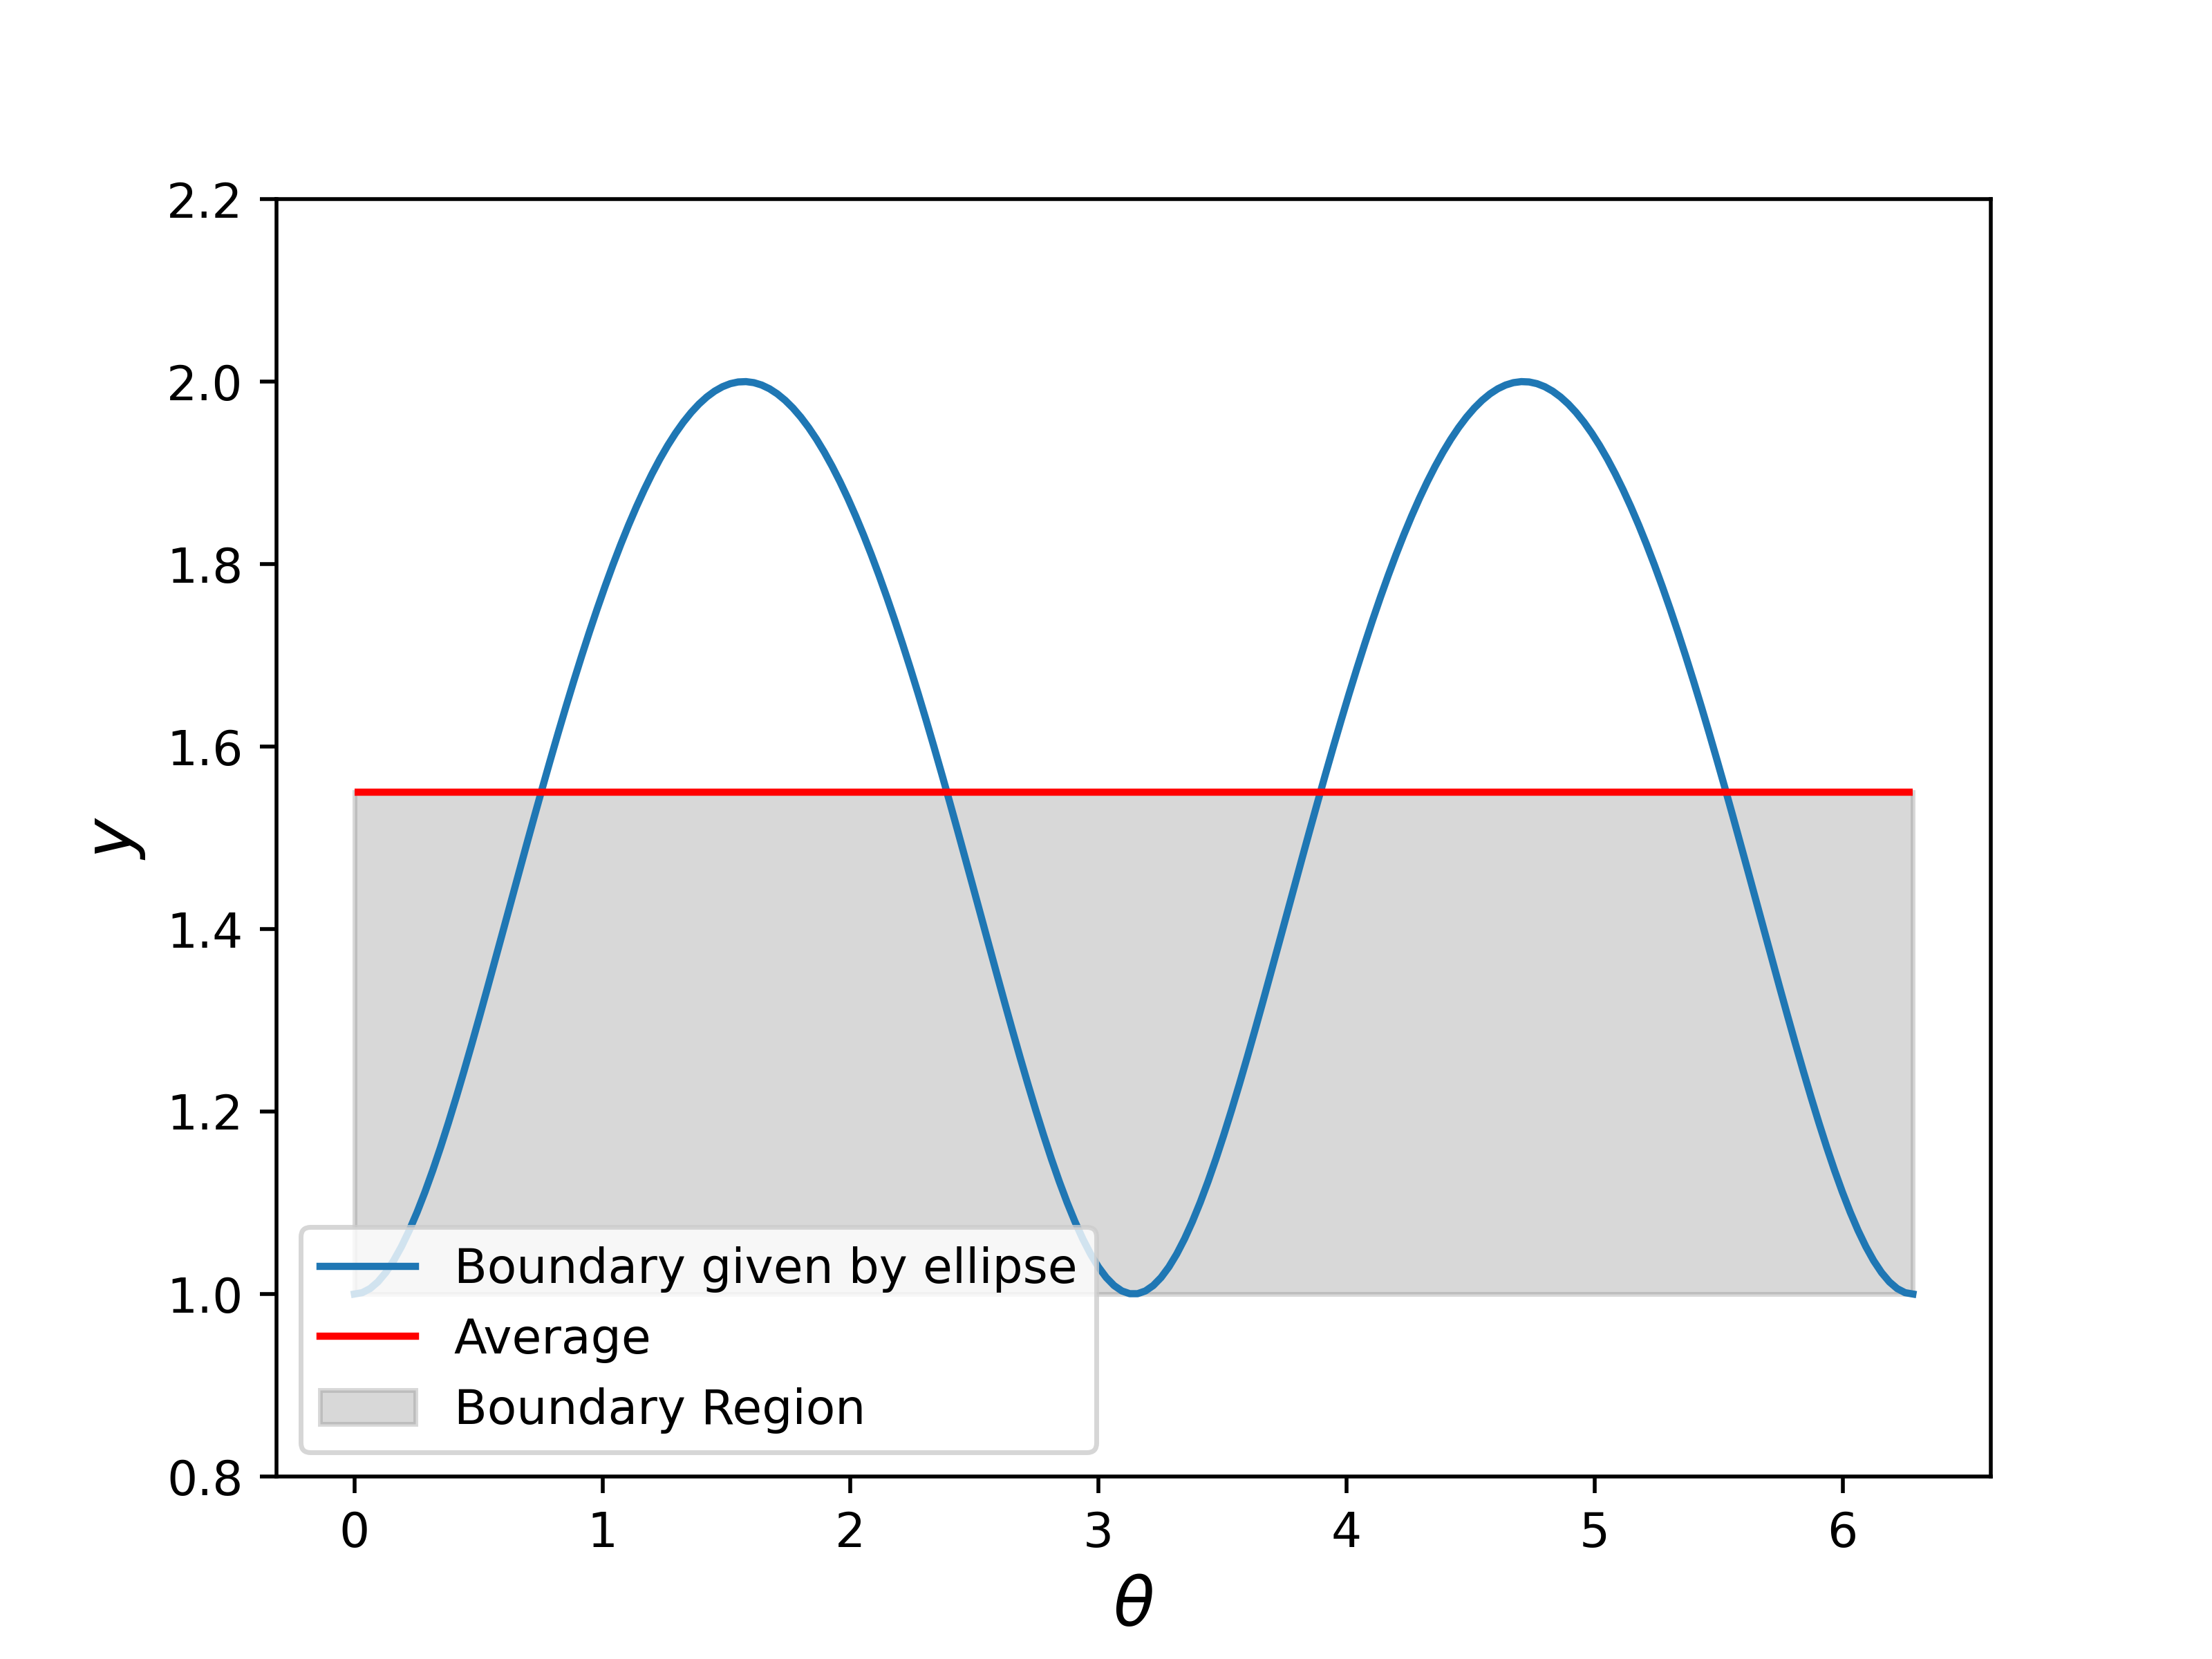
\includegraphics[scale=0.4]{graphics/average_boundary.png}
    \caption{Illustration of methodology for redistributing boundary-accumulated 
    probability mass based on the geometric average boundary distance of an elliptical cell.}
    \label{fig:average_boundary}
\end{figure}

The average was calculated as $\bar{y} = \frac{1}{2\pi}\int_{0}^{2\pi}\sqrt{a^2\sin^2(\theta) + b^2\cos^2(\theta)}$,
where the integrand corresponds to the wall distance function previously defined in \eqref{eq:wall_dist_funcs}.
The resulting adjusted marginal distribution is given in Figure \ref{fig:model_3_modified_hist}.

\begin{figure}[htbp]
    \centering
    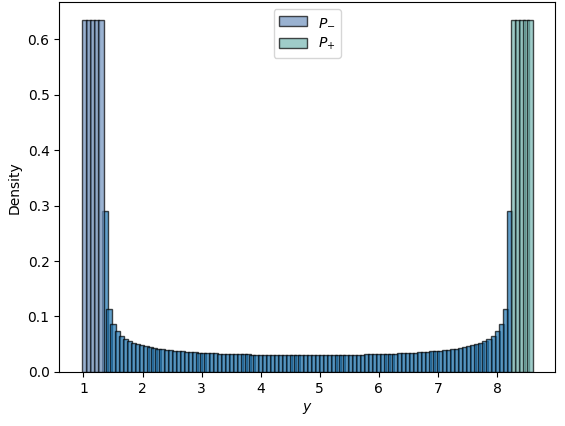
\includegraphics[scale=0.4]{graphics/model_3_with_shape_hist.png}
    \caption{Marginal distribution after redistributing Model 3's boundary-accumulated probability mass according to the cell
    shape.}
    \label{fig:model_3_modified_hist}. 
\end{figure}

Finally, we compared the marginal distributions from Model 1, Model 2 and the modified version of Model 3.
These distributions, generated with identical parameters for consistency, are shown in 
Figure \ref{fig:model_comparisons}.

\begin{figure}[htbp]
    \centering
    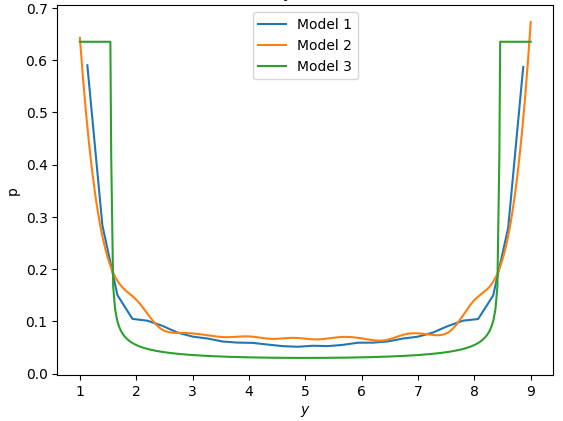
\includegraphics[scale=0.4]{graphics/model_comparisons.png}
    \caption{Comparison of Marginal PDFs from Model 1, Model 2, and the shape-adjusted Model 3.}
    \label{fig:model_comparisons}. 
\end{figure}

From Figure \ref{fig:model_comparisons}, Models 1 and 2 show close alignment, suggesting that additional hydrodynamic
terms in Model 2 may have a relatively minor effect on boundary accumulation under the conditions investigated here.
Further investigation through additional simulations and parameter variations is recommended to comprehensively 
understand the conditions under which hydrodynamic interactions significantly influence the observed cell behavior.

In contrast, Model 3 assigns more probability mass at the boundaries compared to Models 1 and 2. This discrepancy 
suggests that the simplistic bonudary interactions in Model 3 may overestimate the boundary accumulatino effect.

For future work, several extensions can be considered:

\begin{itemize}
    \item Investigate imposing Robin boundary conditions to more accurately capture 
    interactions between cells and boundaries.
    \item Adjusting the cell's centre of rotation, which may usbstantially influence boundary accumulation
    phenomena, as is expored in \cite{chen2021shape}.
    \item Investigating the effects of alternative cell shapes beyond ellipses to generalise the results
    \item Exploring boundary accumulation behaviour near complex boundaries or obstacles, such as circular or 
    irregular shapes within the channel.
    \item Considering collective interactions among the multiple cells to understand how inter-cellular dynamics affect 
    boundary accumulation. 
\end{itemize}





% \section{Modelling UK Renewable Energy Site Locations}\label{sec:3}
% \input{sections/section3.tex}
% \section{Conclusion}\label{sec:conclusion}
% In this report, we investigated several stochastic models aiming to capture the 
boundary-accumulation behavior commonly observed in swimming microorganisms. 
We analyzed three distinct modeling approaches: a purely diffusive model, a model incorporating hydrodynamic interactions with the channel walls, and a piecewise-deterministic Markov process (PDMP) model that explicitly describes boundary capture.

Models 1 and 2, both accounting for cell geometry, provided closely aligned marginal distributions, 
suggesting that hydrodynamic interactions may exert a relatively minor influence under the 
conditions studied here. However, additional exploration of parameter spaces and physical 
scenarios remains essential to thoroughly quantify the role of hydrodynamics in these contexts.

In contrast, Model 3 initially treated cells as point particles, 
yielding exaggerated boundary accumulation. Incorporating geometric considerations into Model 
3 led to a more realistic redistribution of boundary probabilities, yet notable differences 
remained compared to Models 1 and 2. This highlights the importance of accounting explicitly 
for cell geometry in accurately modeling boundary interactions.
\printbibliography

\end{document}